\documentclass[thesis_msc.tex]{subfiles}
\begin{document}

\chapter{FFA pipeline} \label{Chapter:FFA_c}
 	\section{Pulsar surveys}
        \subsection{Previous pulsar survey } \label{survey}
        \paragraph{} After the discovery of the first pulsar by \citep{HEWISH1968}, several of pulsar surveys were initiated. The first generation of pulsar surveys could inspect mainly within the low frequencies range with small bandwidth and frequency resolution. An example of these surveys is Molonglo transit survey \citep{Large:1968:mi}, \citep{Vaughan:1970:lm}, and \citep{Davies:1970:lm} observing using Molonglo telescope located in New South Wales, Australia. This survey, however, was inefficient regarding the detection of high DM pulsars due to the fact that the scattering effect is more prominent at low frequency. Moreover, this survey used bandwidth of 4 MHz with only 2 channels, introducing larger inter-channel DM smearing which could not be corrected using incoherent de-dispersion. The sensitivity of this telescope is quite low due to the narrow bandwidth and short observation time (15 s). This survey observed around 22980 square degree in the sky. The data suggests that pulsars are likely to be located in the Galactic plane. 
        %introduces high sensitivity using Arecibo 305 m telescope. This survey  observed using 430 MHz with 8 MHz bandwidth with 32 channels leading to the discoveries of the Hulse-Taylor pulsar. The most successful in term of the number of discovered pulsar in the beginning pulsar search is the second Molonglo survey \citep{Manchester:1978:rl} which discovered 155 pulsars. As all of these pulsar surveys used low frequency observation ($\sim$ 400 MHz), these survey is bias on high DM pulsar especially on the Galactic plane.  
        
        \paragraph{} The new era of pulsar survey began in the late 1980, when people started  to observe pulsars at a relatively high frequency (1.4 GHz), a practice that takes advantage of the reduction in scattering effect from ISM (\cite{johnston1992high} and \cite{clifton1992high}). However, as mentioned before, pulsar signal is normally weaker at high frequency because it has negative spectral index \citep{bates2013pulsar}. As the signal is weaker in high frequency, the observation time needed is also longer to collect more pulses and leads to longer processing time. Moreover, the angular resolution for high frequency observation is smaller than low frequency, as seen in Equation \ref{angular_res}. As a result, the pulsar survey in high frequency needs more pointings than a low-frequency survey to cover the same region in the sky. 
        
        \paragraph{} Commissioning of the multibeam receiver at Parks telescope \citep{staveley1997hi} opened up a new possibility of pulsar survey at high frequency. The multibeam receiver is capable of observing 13 different patches of the sky simultaneously \citep{staveley1997hi} to compensate for the disadvantage of having smaller angular resolution from observing at high frequency. An example of the survey using multibeam receiver is Parkes multibeam pulsar survey (PMPS). The PMPS is the most successful pulsar survey in the history, discovering over $30 \%$ of all known pulsars with $t_{samp}=0.25 ms$ \cite{camilo2000parkes} and bandwidth of $288$ MHz  \citep{manchester2001parkes}, observing at 1374 MHz. The PMPS observation time is 2100s.  The FFA was applied to the PMPS, leading to the discovery of PSR J1001-5939 with a period of 7.7 s \citep{Faulkner2004} and \citep{lorimer2006parkes}. After that, the implementation of FPGA and digital filterbanks made it possible to do observations in high time and high frequency resolution. An example from these types of survey is the PALFA pulsar survey \citep{cordes2006arecibo} using the 305 m radio telescope at Arecibo. The PALFA survey has their own FFA pipeline, which is in an ongoing process. The preliminary result can be found in  \cite{parent2018implementation} with the results similar to \cite{cameron2017investigation}. Another example of a survey with high time resolution is the High Time Resolution Universe Survey (HTRU).
        
        \subsection{The High Time Resolution Universe survey}
		\paragraph{} The High Time Resolution Universe Survey (HTRU) is a project that consisted of two blind pulsar surveys, the northern (HTRU-N) and southern (HTRU-S) survey. Combining these two surveys will lead us to the most sensitive all-sky pulsar survey at 1.4GHz. The HTRU-N began the survey campaign in 2011 and is still in process. The HTRU-S uses the Parkes 64-m radio telescope located north of Parkes, New South Wales, Australia. The HTRU-S data collecting began in 2011 and finished in 2014. The HTRU-S survey is divided into three regions by the Galactic latitude, as shown in Figure \ref{HTRU_map}. In this work, only low lat survey ($|b|<3.5^o$) will be mentioned. More information about other surveys can be found in \cite{Andrew} and \cite{keith2010high}. The HTRU-S used the Parks Multibeam receiver which consists of 13 feeds producing 13 telescope beams on the sky. Beam patterns on the sky are shown in Figure \ref{HTRU_beam}.  The HTRU-S low lat has the longest observation time compared to other HTRU surveys ($t_{obs}$=4320 s) with $t_{samp}$ =64 $\mu s$ containing $2^{26}$ samples per observation. Longer observation time means more pulses, which is necessary for finding a slow pulsar that emits fewer pulses compared to a fast pulsar in the same time length. The central frequency $f_c$ is located at 1352 MHz with a bandwidth ($\Delta f$) of 340 MHz, separated into 870 channels \citep{keith2010high}. The HTRU-S is a huge improvement from the PMPS due to a finer sampling time, frequency channels, and also longer integration time. Some highlighted discoveries from the HTRU-S low lat included PSR J1101-6424, a recycled pulsar with a massive WD companion, PSR J1847-0427, a pulsar with wide pulse shape that almost entire pulse phase \citep{ng2015high}, and the most accelerated binary pulsar J1757-1854 \citep{cameron2018high}. However, the remaining question is, do we detect all the slow pulsars in the HTRU-S Low lat data? In this work, I applied acceleration-FFA search to the HTRU-S low lat survey data and tried to answer this question. %Since FFA is focused in this work, we will talk only detailed about FFA here. 
        
        \begin{figure}[h!] 
\centering
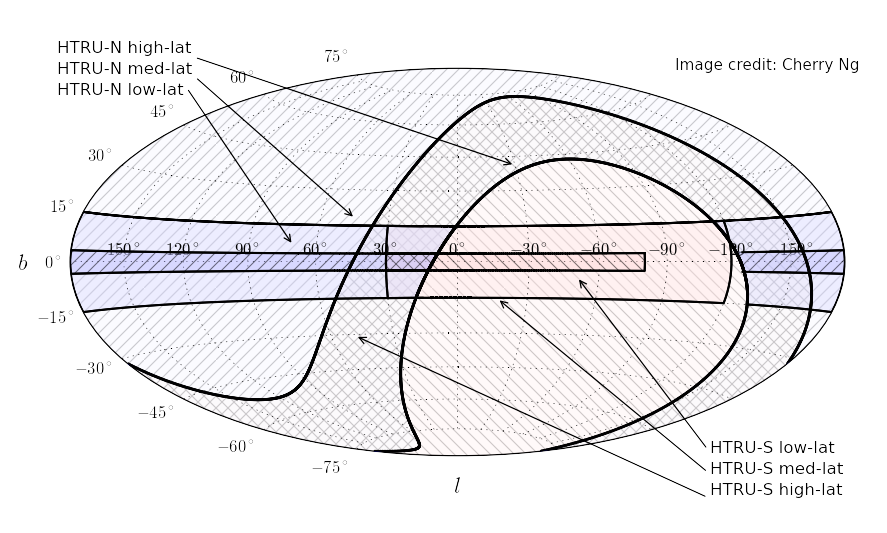
\includegraphics[width=0.7\textwidth]{figures/HTRU-sky-3regions.png}
\caption{The sky coverage of different HTRU surveys. Image obtained from Cherry Ng.}
\label{HTRU_map}
\end{figure}

\begin{figure}[h!]
\centering
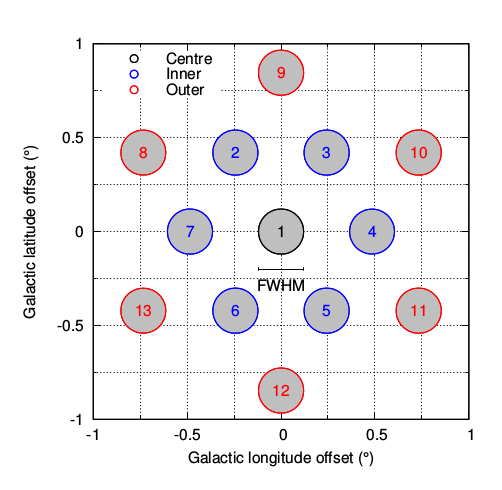
\includegraphics[width=0.650\textwidth]{figures/beampattern}
\caption{Diagram of 13 beams pattern of Parkes telescope with multibeam receiver. FWHM in this case is the angular resolution as shown in Equation \ref{angular_res}. Image from Cherry Ng.}\label{HTRU_beam}
\end{figure}

\section{The FFA pipeline}
\paragraph{} In this work, the maximum search period range is constrained by the assumption that, to detect a pulsar in the FFA, ten pulses are enough to detect the pulsar. As a result, the maximum search period in this work is 430s or $10\%$ of the integration time. The FFA needs more search trials for shorter periods, as shown in Table \ref{FFA_step}, which means longer processing time. The minimum search period needs to be selected carefully. In this work, I used the shortest period that gives a reasonable computational time (less than 12 hours), which is 0.131 s. In addition,  to create a pulse profile, the  minimum searching period needs to be smaller than $bins \cdot t_{samp}$. For profile bins of 128, this condition allows us to perform huge down sampling with a factor of 16 from the original $t_{samp}$ ($64~\mu~s$), which gives minimum search period of 0.131s. The search is divided into 12 different search steps as each of the search step changes every time as the maximum period search follows the condition that $P_{max}=2 P_{min}$ as shown in Table \ref{FFA_step}.       

%\paragraph{} The one of situation that the signal of the pulsar can be lost in FFA search is when the delay time across the whole bandwidth or observation time exceeds one profile bin as Figure \ref{diag}. As a result, the diagonal DM step (as Equation \ref{dm_step_dig}) and acceleration step (as Equation \ref{acc_step}) is used. Using parameter in this survey ($t_{obs},f_c,\delta f,t_{same}$), $DM_0$ and $a_0$ are determined as 3 $pc cm^{-3}$ and 1 $m/s^2$ respectively. Thus, when the search step change as period getting twice longer, the acceleration and DM step also change with the same factor. The maximum search DM is chosen from the fact that, HTRU-S low lat is the data from the densest region in the Galaxy. The maximum DM in this case is 3072 $cm^{-3}pc$. The maximum DM is originated from the nearest common factor for each DM step to 3000 $cm^{-3}pc$. DM of 3000 $cm^{-3}pc$  originate from the DM range of HTRU-S Low lat FFT pipeline DM range \citep{ng2015high}. The maximum acceleration range is calculated from the maximum acceleration produced by pulse-BH binary with $m_c=37 M_{\odot}$ which is $128 m/s^2$. The overall detail of this pipeline can be found at \ref{flow}. As DM and acceleration step changes with the searching period, this method demonstrates that acceleration search with FFA is highly optimised because the pipeline can skip some DM and a step when period got longer without losing any S/N. Moreover, De-dispersion and time domain re-sampling need to apply only with the finest step. The pipeline will skip some DM, and a step when searching period getting longer as shown in Figure \ref{FFA_process}. After reaching the maximum DM and acceleration, the pipeline will search for the periodicity in the time series that correspond to DM of 0 and 3072 $cm^{-3} pc$ and acceleration of -128.0,0, and 128.0 $m/s^2$ as show in Table\ref{FFA_step}.
\paragraph{} One of the situations that the signal of the pulsar is lost in the FFA search is when the delay time across the whole bandwidth exceeds one profile bin, as shown in Figure \ref{diag}. As a result, the diagonal DM step, as shown in Equation \ref{dm_step_dig}, is used. Using a parameter in this survey ($t_{obs},f_c,t_{samp}$), $DM_0$ is determined as 3 $pc~cm^{-3}$. Thus, when the search step changes as the period is getting twice longer, as shown in the second row in Table \ref{FFA_step} , the DM step also changes with the same factor as the DM step , which is proportional to $Df$ as shown in Equation \ref{dm_step}. The maximum search DM is chosen from the fact that the HTRU-S low lat is the data from the most dense region in the Galaxy, implying a large DM. The maximum DM in this case is 3072 $pc~cm^{-3}$. The maximum DM comes from the nearest common factor for each DM step to 3000 $pc~cm^{-3}$. Otherwise, the number of DM step is not optimised. For example, at searching period range of 2.097125s to 4.194304s, the DM step for this period range is 48 $pc~cm^{-3}$, which gives non-integer number of DM step.   Moreover, the maximum DM of 3000 $pc~cm^{-3}$ is then originated from the DM range of the HTRU-S Low lat FFT pipeline DM range \citep{ng2015high}. The overall detail of this pipeline can be found further as shown in Figure \ref{flow}. As $Df$ changes with searching periods, this method demonstrates that DM search with the FFA is highly optimised because the pipeline can skip some DM steps when searching periods getting longer without losing any S/N. As a result, De-dispersion needs to be applied only with the final step. The pipeline will skip some of the DM steps when searching period is getting longer as shown in Figure \ref{FFA_process}. After reaching the maximum DM, the pipeline will search for the periodicity in the time series that corresponds to the DM of 0 and 3072 $pc~cm^{-3}$ , as shown in Table\ref{FFA_step}. For acceleration search, Equation \ref{acc_step} shows that the first acceleration step is 1 $m/s^2$, as searching periods are getting twice longer, the pipeline performed down sampling with a factor of two, making the acceleration step twice larger, as shown in Table \ref{FFA_step}.  The maximum acceleration range is calculated from the maximum acceleration, produced by pulse-BH binary with $m_c=37 M_{\odot}$ at orbital period of 12 hours, which is $^+_-128 m/s^2$ for observation time of 4320 s. The orbital period came from the ``10 percent rule" where the constant acceleration condition is applied when the observation time is 10 percent of the orbital period. 


\begin{figure}[h] \centering
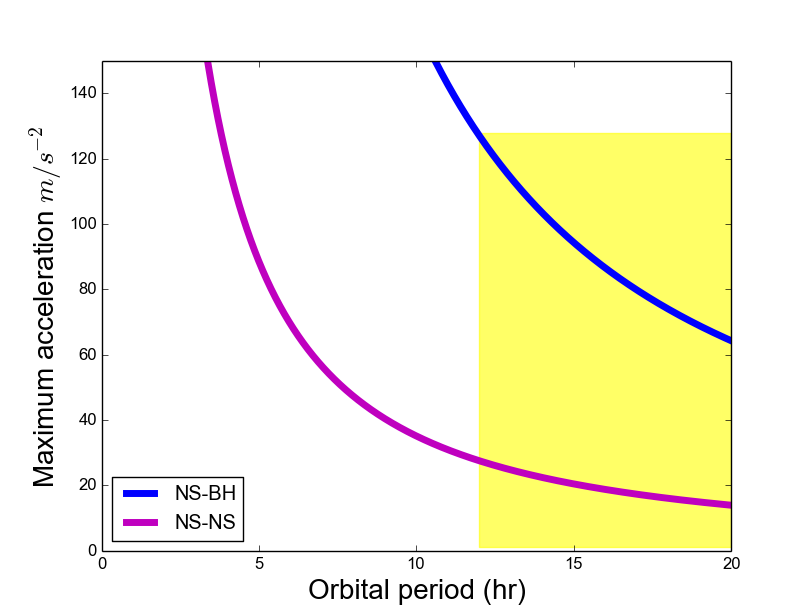
\includegraphics[width=1.0\textwidth]{figures/acc_plot.png}
\caption{The Maximum acceleration for different orbital periods ($P_{obs}$) for pulsar with 37 and 1.4 $M_\odot$ companions. The yellow regions correspond to acceleration and orbital period where constant acceleration approximation is the most effective for an observation time of 4320 s. }
\label{Fig:acc_range}
\end{figure}


\paragraph{} The pipeline used the  \textit{PRESTO} package to mask out the RFI, using the \textit{rfifind} routine. The de-dispersion process has been done with the \textit{PRESTO} . The time series will be re-sampled by python package \textit{sigpyproc}. The FFA search and sifting in period and DM part have been done in \textit{riptide} \footnote{https://bitbucket.org/vmorello/riptide/src/master}. The sifting for acceleration domain has been done in this pipeline by grouping candidates that have period and DM in the same search bins. Then, the pipeline will search for the strongest candidate. 
\\

       \begin{table}[h!]  \centering
        \caption{The FFA searching for the period includes the steps from 1.0 to 539.90 s periodic signal. The minimum and the maximum searching bins are set to be 128 and 256 respectively. The original sampling time $t_{samp}$ is 1.024 ms. The sampling time for each period is selected from the fact that $t_{samp}$ for each period needs to be at least $1/bins_{min}$, which can introduce a huge down sampling factor $Df$. }
\label{FFA_step}
\resizebox{\textwidth}{!}{%
\begin{tabular}{|l|l|l|l|l|l|l|l|l|l|l|l|}
\hline
i & Df & $t_{samp}$ & $N_B$ & $P_{min}$ & $P_{max}$ & $a_{theory}$ & $a_i$ & $DM_i$ & Na & $N_{dm}$ & $n_{trial}$ \\ \hline
1 & 1 & 0.001024 & 128 & 0.131072 & 0.262144 & 1.053497942 & 1 & 3 & 257 & 1024 & 33685504 \\ \hline
2 & 2 & 0.002048 & 128 & 0.262144 & 0.524288 & 2.106995885 & 2 & 6 & 129 & 512 & 8454144 \\ \hline
3 & 4 & 0.004096 & 128 & 0.524288 & 1.048576 & 4.21399177 & 4 & 12 & 65 & 256 & 2129920 \\ \hline
4 & 8 & 0.008192 & 128 & 1.048576 & 2.097152 & 8.427983539 & 8 & 24 & 33 & 128 & 540672 \\ \hline
5 & 16 & 0.016384 & 128 & 2.097152 & 4.194304 & 16.85596708 & 16 & 48 & 17 & 64 & 139264 \\ \hline
6 & 32 & 0.032768 & 128 & 4.194304 & 8.388608 & 33.71193416 & 32 & 96 & 9 & 32 & 36864 \\ \hline
7 & 64 & 0.065536 & 128 & 8.388608 & 16.777216 & 67.42386831 & 64 & 192 & 5 & 16 & 10240 \\ \hline
8 & 128 & 0.131072 & 128 & 16.777216 & 33.554432 & 134.8477366 & 128 & 384 & 3 & 8 & 3072 \\ \hline
9 & 256 & 0.262144 & 128 & 33.554432 & 67.108864 & 269.6954733 & 256 & 768 & 2 & 4 & 1024 \\ \hline
10 & 512 & 0.524288 & 128 & 67.108864 & 134.217728 & 432.0 & 512 & 1536 & 1 & 2 & 256 \\ \hline
11 & 1024 & 1.048576 & 128 & 134.217728 & 268.435456 & 1078.781893 & 512 & 3072 & 1 & 2 & 256 \\ \hline
12 & 2048 & 2.097152 & 128 & 268.435456 & 430 & 2157.563786 & 512 & 3072 & 1 & 2 & 256 \\ \hline
\end{tabular}%
}
\end{table}

    \begin{figure}[h!]
\centering
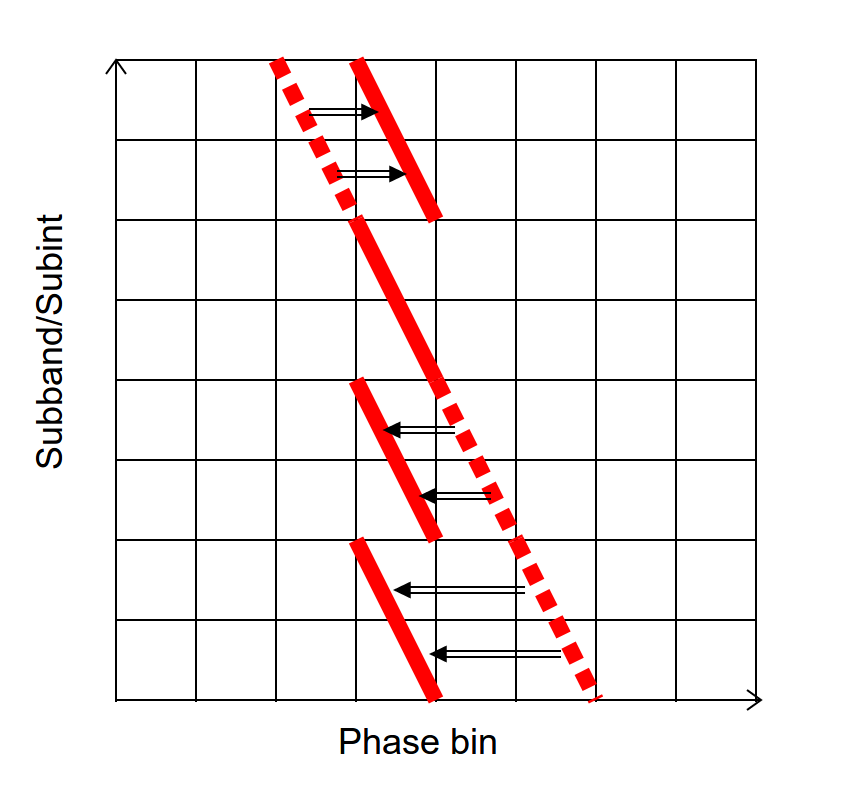
\includegraphics[width=0.5\textwidth]{figures/4bins.png}
\caption{Example of incoherent de-dispersion or time domain re-sampling in the case of diagonal DM/acceleration in narrow bandwidth/short $t_{obs}$.}\label{diag}
\end{figure}

     
     




\tikzset{every picture/.style={line width=0.75pt}} %set default line width to 0.75pt        

\begin{figure}[h!]
\centering


\tikzset{every picture/.style={line width=0.50pt}} %set default line width to 0.75pt        

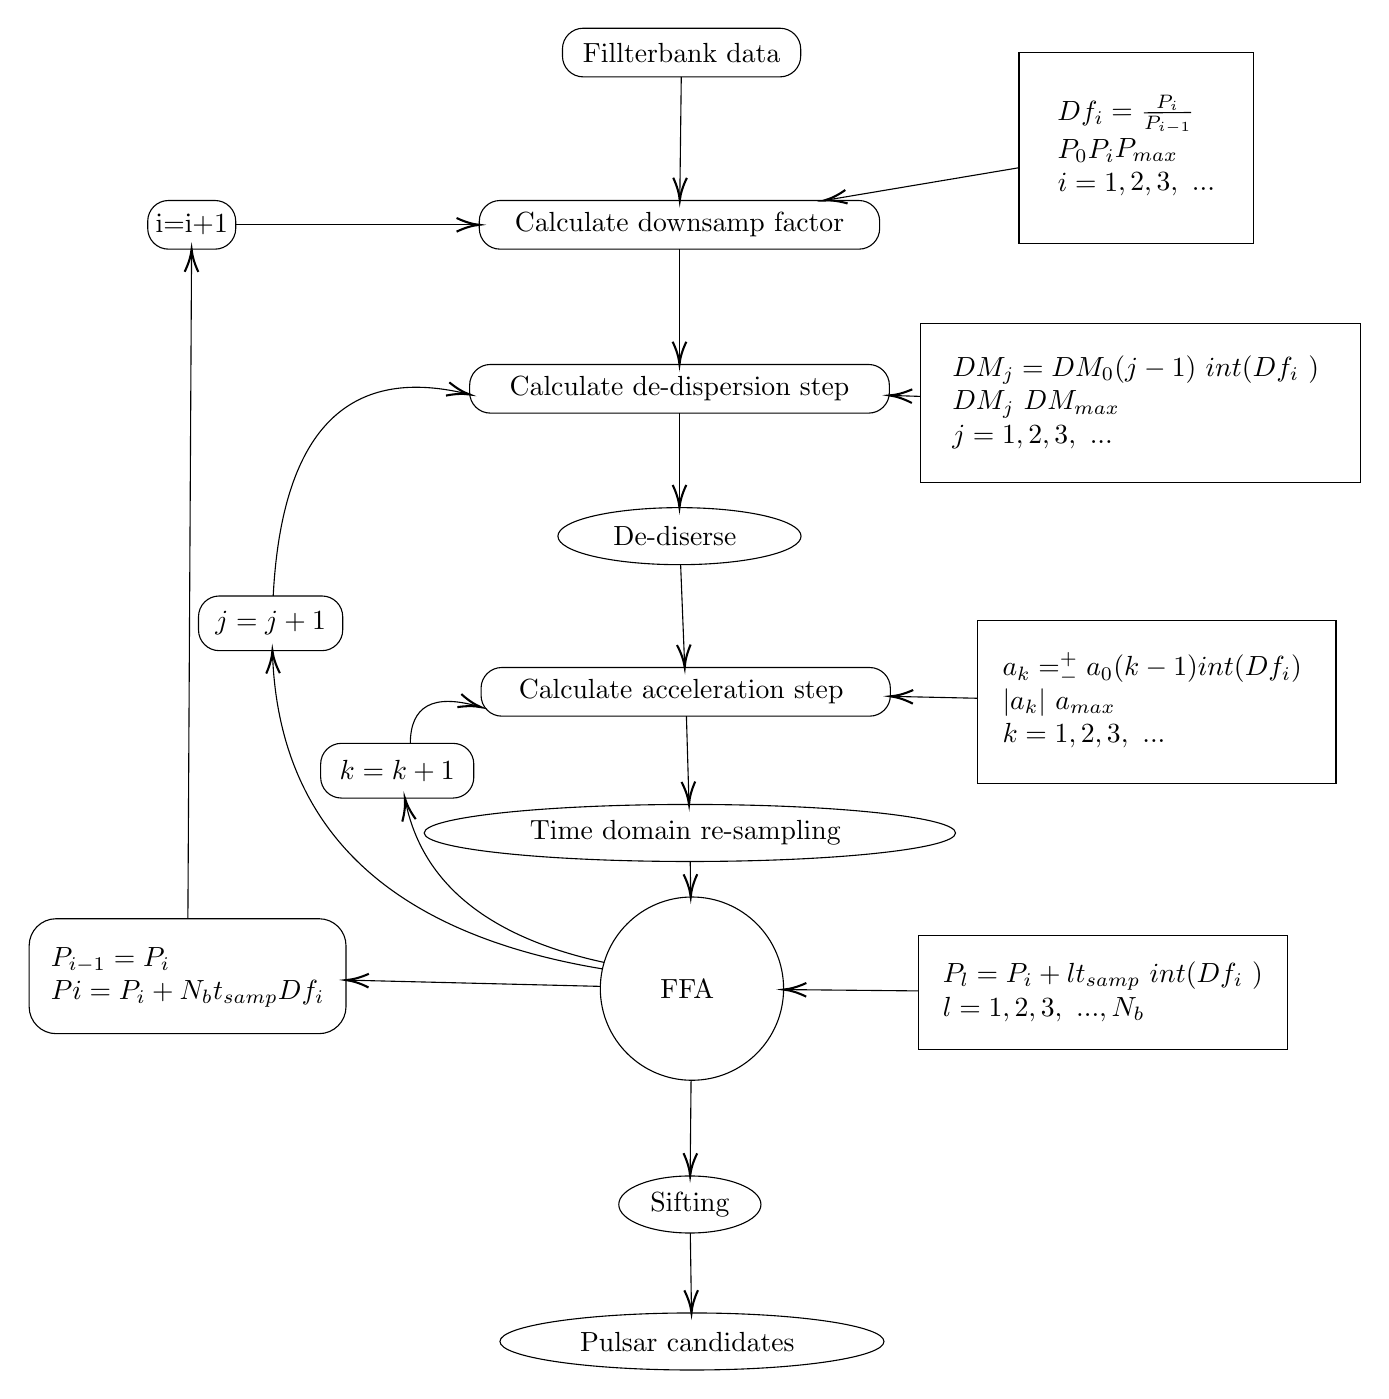
\begin{tikzpicture}[x=0.75pt,y=0.75pt,yscale=-1,xscale=1]
%uncomment if require: \path (0,658); %set diagram left start at 0, and has height of 658


% Text Node
\draw    (272.62,12.28) .. controls (272.62,6.76) and (277.09,2.28) .. (282.62,2.28) -- (377.4,2.28) .. controls (382.92,2.28) and (387.4,6.76) .. (387.4,12.28) -- (387.4,15.72) .. controls (387.4,21.24) and (382.92,25.72) .. (377.4,25.72) -- (282.62,25.72) .. controls (277.09,25.72) and (272.62,21.24) .. (272.62,15.72) -- cycle  ;
\draw (330,14) node  [align=left] {Fillterbank data};
% Text Node
\draw    (232.55,95.28) .. controls (232.55,89.76) and (237.03,85.28) .. (242.55,85.28) -- (415.45,85.28) .. controls (420.97,85.28) and (425.45,89.76) .. (425.45,95.28) -- (425.45,98.72) .. controls (425.45,104.24) and (420.97,108.72) .. (415.45,108.72) -- (242.55,108.72) .. controls (237.03,108.72) and (232.55,104.24) .. (232.55,98.72) -- cycle  ;
\draw (329,97) node  [align=left] {Calculate downsamp factor};
% Text Node
\draw    (492.57,14.15) -- (605.42,14.15) -- (605.42,105.87) -- (492.57,105.87) -- cycle  ;
\draw (549,60) node [rotate=-359.6]  {$ \begin{array}{l}
Df_{i} =\frac{P_{i}}{P_{i-1}} \ \\
P_{0} \leqq P_{i} \leqq P_{max}\\
i=1,2,3,\ ...
\end{array}$};
% Text Node
\draw    (227.9,174.28) .. controls (227.9,168.76) and (232.38,164.28) .. (237.9,164.28) -- (420.12,164.28) .. controls (425.64,164.28) and (430.12,168.76) .. (430.12,174.28) -- (430.12,177.72) .. controls (430.12,183.24) and (425.64,187.72) .. (420.12,187.72) -- (237.9,187.72) .. controls (232.38,187.72) and (227.9,183.24) .. (227.9,177.72) -- cycle  ;
\draw (329,176) node  [align=left] {Calculate de-dispersion step};
% Text Node
\draw    (444.98,144.72) -- (657.03,144.72) -- (657.03,221.28) -- (444.98,221.28) -- cycle  ;
\draw (551,183) node   {$ \begin{array}{l}
DM_{j} =DM_{0}( j-1) \ int( Df_{i} \ ) \ \\
DM_{j} \ \leqq DM_{max}\\
j=1,2,3,\ ...
\end{array}$};
% Text Node
\draw    (329, 247) circle [x radius= 58.57, y radius= 13.74]   ;
\draw (329,247) node  [align=left] {De-diserse };
% Text Node
\draw    (233.4,320.28) .. controls (233.4,314.76) and (237.88,310.28) .. (243.4,310.28) -- (420.6,310.28) .. controls (426.12,310.28) and (430.6,314.76) .. (430.6,320.28) -- (430.6,323.72) .. controls (430.6,329.24) and (426.12,333.72) .. (420.6,333.72) -- (243.4,333.72) .. controls (237.88,333.72) and (233.4,329.24) .. (233.4,323.72) -- cycle  ;
\draw (332,322) node  [align=left] {Calculate acceleration step };
% Text Node
\draw    (472.68,287.7) -- (645.32,287.7) -- (645.32,366.3) -- (472.68,366.3) -- cycle  ;
\draw (559,327) node   {$ \begin{array}{l}
a_{k} =^{+}_{-} a_{0}( k-1) int( Df_{i}) \ \\
|a_{k} |\ \leqq a_{max}\\
k=1,2,3,\ ...
\end{array}$};
% Text Node
\draw    (334.01, 390) circle [x radius= 128, y radius= 13.74]   ;
\draw (334,390) node  [align=left] {Time domain re-sampling };
% Text Node
\draw    (335.01, 465) circle [x radius= 44.15, y radius= 44.15]   ;
\draw (335,465) node  [align=left] { \ \ \ \ \ FFA \ \ \ \ \ };
% Text Node
\draw    (444.18,439.47) -- (621.83,439.47) -- (621.83,494.53) -- (444.18,494.53) -- cycle  ;
\draw (533,467) node   {$ \begin{array}{l}
P_{l} =P_{i} +lt_{samp} \ int( Df_{i} \ )\\
l=1,2,3,\ ...,N_{b}
\end{array}$};
% Text Node
\draw    (334, 569) circle [x radius= 34.25, y radius= 13.74]   ;
\draw (334,569) node  [align=left] {Sifting};
% Text Node
\draw    (15.67,444.32) .. controls (15.67,437.14) and (21.49,431.32) .. (28.67,431.32) -- (155.33,431.32) .. controls (162.51,431.32) and (168.33,437.14) .. (168.33,444.32) -- (168.33,473.7) .. controls (168.33,480.88) and (162.51,486.7) .. (155.33,486.7) -- (28.67,486.7) .. controls (21.49,486.7) and (15.67,480.88) .. (15.67,473.7) -- cycle  ;
\draw (92,459) node [rotate=-359.88]  {$ \begin{array}{l}
P_{i-1} =P_{i}\\
Pi=P_{i} +N_{b} t_{samp} Df_{i}
\end{array}$};
% Text Node
\draw    (72.8,95.28) .. controls (72.8,89.76) and (77.28,85.28) .. (82.8,85.28) -- (105.2,85.28) .. controls (110.72,85.28) and (115.2,89.76) .. (115.2,95.28) -- (115.2,98.72) .. controls (115.2,104.24) and (110.72,108.72) .. (105.2,108.72) -- (82.8,108.72) .. controls (77.28,108.72) and (72.8,104.24) .. (72.8,98.72) -- cycle  ;
\draw (94,97) node  [align=left] {i=i+1};
% Text Node
\draw    (156.12,356.82) .. controls (156.12,351.29) and (160.59,346.82) .. (166.12,346.82) -- (219.9,346.82) .. controls (225.42,346.82) and (229.9,351.29) .. (229.9,356.82) -- (229.9,363.18) .. controls (229.9,368.71) and (225.42,373.18) .. (219.9,373.18) -- (166.12,373.18) .. controls (160.59,373.18) and (156.12,368.71) .. (156.12,363.18) -- cycle  ;
\draw (193,360) node [rotate=-359.88]  {$k=k+1$};
% Text Node
\draw    (97.27,285.82) .. controls (97.27,280.29) and (101.74,275.82) .. (107.27,275.82) -- (156.75,275.82) .. controls (162.27,275.82) and (166.75,280.29) .. (166.75,285.82) -- (166.75,292.17) .. controls (166.75,297.69) and (162.27,302.17) .. (156.75,302.17) -- (107.27,302.17) .. controls (101.74,302.17) and (97.27,297.69) .. (97.27,292.17) -- cycle  ;
\draw (132,289) node [rotate=-359.88]  {$j=j+1$};
% Text Node
\draw    (335.01, 635) circle [x radius= 92.52, y radius= 13.74]   ;
\draw (335,635) node  [align=left] {Pulsar candidates };
% Connection
\draw    (329.86,25.72) -- (329.17,83.28) ;
\draw [shift={(329.14,85.28)}, rotate = 270.69] [color={rgb, 255:red, 0; green, 0; blue, 0 }  ][line width=0.75]    (10.93,-3.29) .. controls (6.95,-1.4) and (3.31,-0.3) .. (0,0) .. controls (3.31,0.3) and (6.95,1.4) .. (10.93,3.29)   ;

% Connection
\draw    (492.57,69.49) -- (400.64,84.95) ;
\draw [shift={(398.67,85.28)}, rotate = 350.45] [color={rgb, 255:red, 0; green, 0; blue, 0 }  ][line width=0.75]    (10.93,-3.29) .. controls (6.95,-1.4) and (3.31,-0.3) .. (0,0) .. controls (3.31,0.3) and (6.95,1.4) .. (10.93,3.29)   ;

% Connection
\draw    (329,108.72) -- (329,162.28) ;
\draw [shift={(329,164.28)}, rotate = 270] [color={rgb, 255:red, 0; green, 0; blue, 0 }  ][line width=0.75]    (10.93,-3.29) .. controls (6.95,-1.4) and (3.31,-0.3) .. (0,0) .. controls (3.31,0.3) and (6.95,1.4) .. (10.93,3.29)   ;

% Connection
\draw    (444.98,179.66) -- (432.12,179.25) ;
\draw [shift={(430.12,179.19)}, rotate = 361.81] [color={rgb, 255:red, 0; green, 0; blue, 0 }  ][line width=0.75]    (10.93,-3.29) .. controls (6.95,-1.4) and (3.31,-0.3) .. (0,0) .. controls (3.31,0.3) and (6.95,1.4) .. (10.93,3.29)   ;

% Connection
\draw    (329,187.72) -- (329,231.26) ;
\draw [shift={(329,233.26)}, rotate = 270] [color={rgb, 255:red, 0; green, 0; blue, 0 }  ][line width=0.75]    (10.93,-3.29) .. controls (6.95,-1.4) and (3.31,-0.3) .. (0,0) .. controls (3.31,0.3) and (6.95,1.4) .. (10.93,3.29)   ;

% Connection
\draw    (329.55,260.74) -- (331.45,308.28) ;
\draw [shift={(331.53,310.28)}, rotate = 267.71] [color={rgb, 255:red, 0; green, 0; blue, 0 }  ][line width=0.75]    (10.93,-3.29) .. controls (6.95,-1.4) and (3.31,-0.3) .. (0,0) .. controls (3.31,0.3) and (6.95,1.4) .. (10.93,3.29)   ;

% Connection
\draw    (472.68,325.1) -- (432.6,324.22) ;
\draw [shift={(430.6,324.17)}, rotate = 361.26] [color={rgb, 255:red, 0; green, 0; blue, 0 }  ][line width=0.75]    (10.93,-3.29) .. controls (6.95,-1.4) and (3.31,-0.3) .. (0,0) .. controls (3.31,0.3) and (6.95,1.4) .. (10.93,3.29)   ;

% Connection
\draw    (332.34,333.72) -- (333.54,374.26) ;
\draw [shift={(333.6,376.26)}, rotate = 268.32] [color={rgb, 255:red, 0; green, 0; blue, 0 }  ][line width=0.75]    (10.93,-3.29) .. controls (6.95,-1.4) and (3.31,-0.3) .. (0,0) .. controls (3.31,0.3) and (6.95,1.4) .. (10.93,3.29)   ;

% Connection
\draw    (334.18,403.74) -- (334.38,418.86) ;
\draw [shift={(334.41,420.86)}, rotate = 269.24] [color={rgb, 255:red, 0; green, 0; blue, 0 }  ][line width=0.75]    (10.93,-3.29) .. controls (6.95,-1.4) and (3.31,-0.3) .. (0,0) .. controls (3.31,0.3) and (6.95,1.4) .. (10.93,3.29)   ;

% Connection
\draw    (444.18,466.1) -- (381.15,465.47) ;
\draw [shift={(379.15,465.45)}, rotate = 360.58000000000004] [color={rgb, 255:red, 0; green, 0; blue, 0 }  ][line width=0.75]    (10.93,-3.29) .. controls (6.95,-1.4) and (3.31,-0.3) .. (0,0) .. controls (3.31,0.3) and (6.95,1.4) .. (10.93,3.29)   ;

% Connection
\draw    (334.58,509.15) -- (334.15,553.26) ;
\draw [shift={(334.13,555.26)}, rotate = 270.55] [color={rgb, 255:red, 0; green, 0; blue, 0 }  ][line width=0.75]    (10.93,-3.29) .. controls (6.95,-1.4) and (3.31,-0.3) .. (0,0) .. controls (3.31,0.3) and (6.95,1.4) .. (10.93,3.29)   ;

% Connection
\draw    (290.87,463.91) -- (170.33,460.93) ;
\draw [shift={(168.33,460.88)}, rotate = 361.40999999999997] [color={rgb, 255:red, 0; green, 0; blue, 0 }  ][line width=0.75]    (10.93,-3.29) .. controls (6.95,-1.4) and (3.31,-0.3) .. (0,0) .. controls (3.31,0.3) and (6.95,1.4) .. (10.93,3.29)   ;

% Connection
\draw    (92.15,431.32) -- (93.92,110.72) ;
\draw [shift={(93.94,108.72)}, rotate = 450.32] [color={rgb, 255:red, 0; green, 0; blue, 0 }  ][line width=0.75]    (10.93,-3.29) .. controls (6.95,-1.4) and (3.31,-0.3) .. (0,0) .. controls (3.31,0.3) and (6.95,1.4) .. (10.93,3.29)   ;

% Connection
\draw    (115.2,97) -- (230.55,97) ;
\draw [shift={(232.55,97)}, rotate = 180] [color={rgb, 255:red, 0; green, 0; blue, 0 }  ][line width=0.75]    (10.93,-3.29) .. controls (6.95,-1.4) and (3.31,-0.3) .. (0,0) .. controls (3.31,0.3) and (6.95,1.4) .. (10.93,3.29)   ;

% Connection
\draw    (292.71,452.37) .. controls (237.08,440.3) and (205.19,414.51) .. (197.04,375) ;
\draw [shift={(196.68,373.18)}, rotate = 439.46] [color={rgb, 255:red, 0; green, 0; blue, 0 }  ][line width=0.75]    (10.93,-3.29) .. controls (6.95,-1.4) and (3.31,-0.3) .. (0,0) .. controls (3.31,0.3) and (6.95,1.4) .. (10.93,3.29)   ;

% Connection
\draw    (199.31,346.82) .. controls (199.42,328.8) and (210.23,322.84) .. (231.73,328.92) ;
\draw [shift={(233.4,329.41)}, rotate = 196.91] [color={rgb, 255:red, 0; green, 0; blue, 0 }  ][line width=0.75]    (10.93,-3.29) .. controls (6.95,-1.4) and (3.31,-0.3) .. (0,0) .. controls (3.31,0.3) and (6.95,1.4) .. (10.93,3.29)   ;

% Connection
\draw    (133.25,275.82) .. controls (137.39,197.06) and (168.35,164.56) .. (226.14,178.32) ;
\draw [shift={(227.9,178.75)}, rotate = 194.13] [color={rgb, 255:red, 0; green, 0; blue, 0 }  ][line width=0.75]    (10.93,-3.29) .. controls (6.95,-1.4) and (3.31,-0.3) .. (0,0) .. controls (3.31,0.3) and (6.95,1.4) .. (10.93,3.29)   ;

% Connection
\draw    (291.9,455.49) .. controls (188.81,438.42) and (135.81,387.73) .. (132.91,303.44) ;
\draw [shift={(132.87,302.17)}, rotate = 448.37] [color={rgb, 255:red, 0; green, 0; blue, 0 }  ][line width=0.75]    (10.93,-3.29) .. controls (6.95,-1.4) and (3.31,-0.3) .. (0,0) .. controls (3.31,0.3) and (6.95,1.4) .. (10.93,3.29)   ;

% Connection
\draw    (334.21,582.74) -- (334.76,619.26) ;
\draw [shift={(334.79,621.26)}, rotate = 269.13] [color={rgb, 255:red, 0; green, 0; blue, 0 }  ][line width=0.75]    (10.93,-3.29) .. controls (6.95,-1.4) and (3.31,-0.3) .. (0,0) .. controls (3.31,0.3) and (6.95,1.4) .. (10.93,3.29)   ;


\end{tikzpicture}
\caption{Processing flowchart for acceleration search with the FFA pipeline (AFFA). }
\label{flow}
\end{figure}

        
          \begin{figure}[h]
\centering


\tikzset{every picture/.style={line width=0.50pt}} %set default line width to 0.75pt        

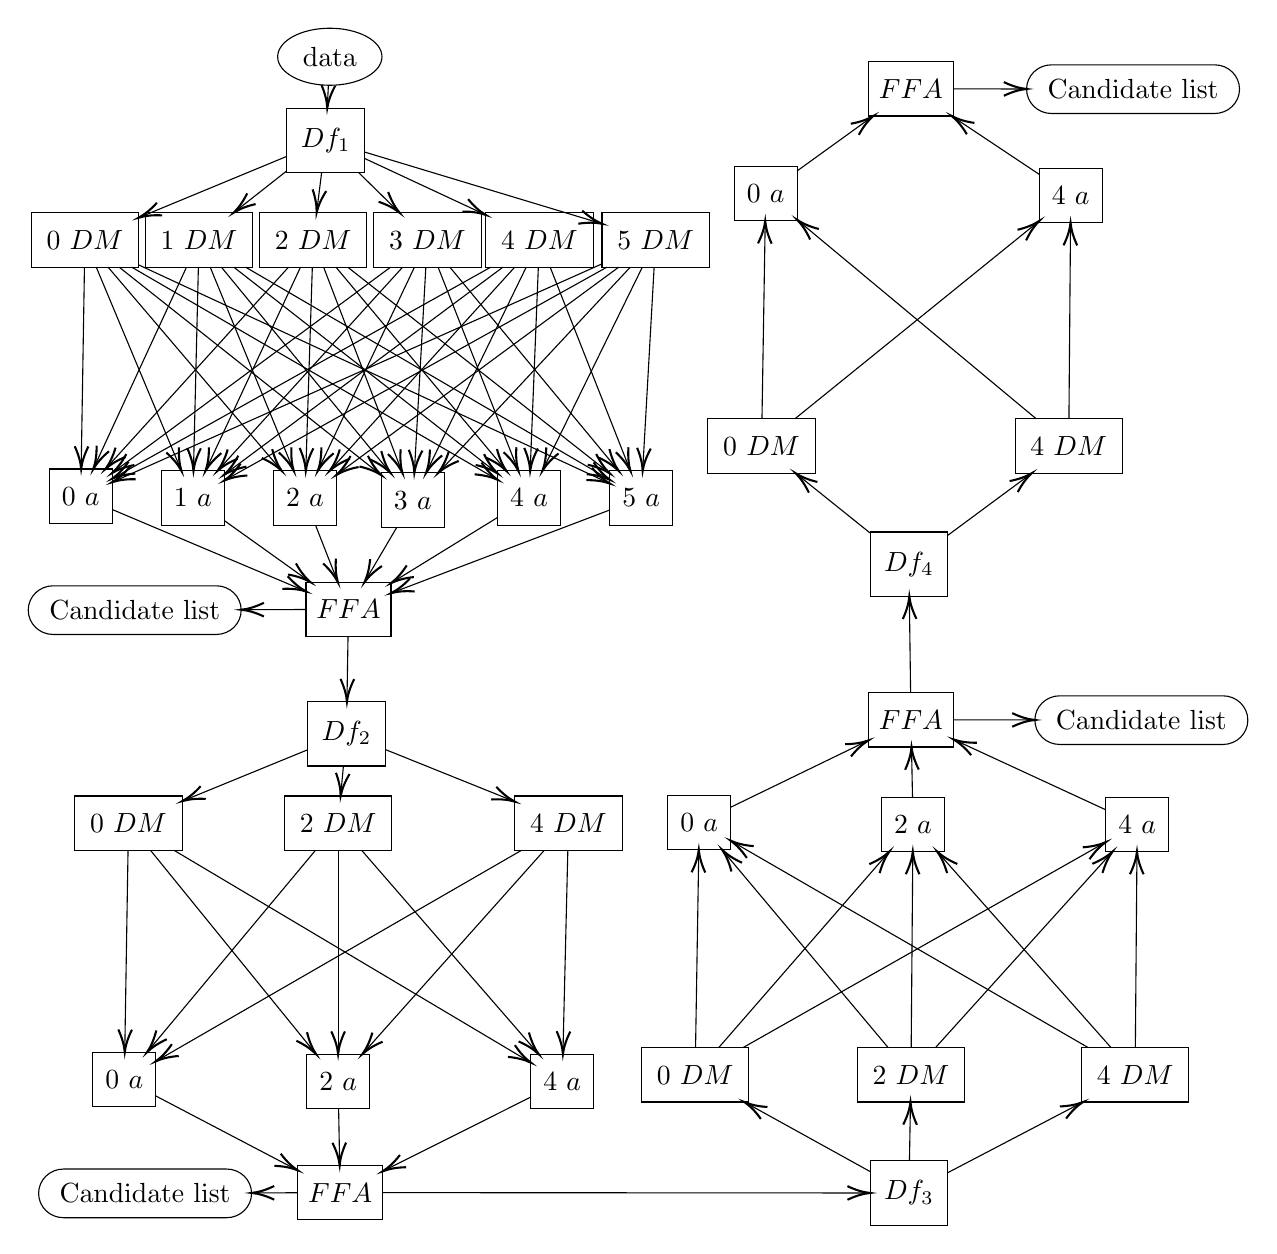
\begin{tikzpicture}[x=0.75pt,y=0.75pt,yscale=-1,xscale=1]
%uncomment if require: \path (0,600.5333251953125); %set diagram left start at 0, and has height of 600.5333251953125


% Text Node
\draw    (149, 16.38) circle [x radius= 25.13, y radius= 13.74]   ;
\draw (149,16.38) node  [align=left] {data};
% Text Node
\draw    (128.32,41.13) -- (165.7,41.13) -- (165.7,72.1) -- (128.32,72.1) -- cycle  ;
\draw (147,56.62) node   {$Df_{1}$};
% Text Node
\draw    (5.15,91.55) -- (56.87,91.55) -- (56.87,117.77) -- (5.15,117.77) -- cycle  ;
\draw (31,104.65) node   {$0\ DM$};
% Text Node
\draw    (115.13,91.55) -- (166.85,91.55) -- (166.85,117.77) -- (115.13,117.77) -- cycle  ;
\draw (141,104.65) node   {$2\ DM$};
% Text Node
\draw    (170.15,91.55) -- (221.87,91.55) -- (221.87,117.77) -- (170.15,117.77) -- cycle  ;
\draw (196,104.65) node   {$3\ DM$};
% Text Node
\draw    (224.15,91.55) -- (275.87,91.55) -- (275.87,117.77) -- (224.15,117.77) -- cycle  ;
\draw (250,104.65) node   {$4\ DM$};
% Text Node
\draw    (280.15,91.55) -- (331.87,91.55) -- (331.87,117.77) -- (280.15,117.77) -- cycle  ;
\draw (306,104.65) node   {$5\ DM$};
% Text Node
\draw    (13.9,215.02) -- (44.12,215.02) -- (44.12,241.23) -- (13.9,241.23) -- cycle  ;
\draw (29,228.12) node   {$0\ a$};
% Text Node
\draw    (121.9,215.9) -- (152.12,215.9) -- (152.12,242.12) -- (121.9,242.12) -- cycle  ;
\draw (137,229) node   {$2\ a$};
% Text Node
\draw    (173.9,216.88) -- (204.12,216.88) -- (204.12,243.1) -- (173.9,243.1) -- cycle  ;
\draw (189,230) node   {$3\ a$};
% Text Node
\draw    (229.9,215.9) -- (260.12,215.9) -- (260.12,242.12) -- (229.9,242.12) -- cycle  ;
\draw (245,229) node   {$4\ a$};
% Text Node
\draw    (283.9,215.9) -- (314.12,215.9) -- (314.12,242.12) -- (283.9,242.12) -- cycle  ;
\draw (299,229) node   {$5\ a$};
% Text Node
\draw    (60.15,91.55) -- (111.87,91.55) -- (111.87,117.77) -- (60.15,117.77) -- cycle  ;
\draw (86,104.65) node   {$1\ DM$};
% Text Node
\draw    (67.88,215.9) -- (98.1,215.9) -- (98.1,242.12) -- (67.88,242.12) -- cycle  ;
\draw (83,229) node   {$1\ a$};
% Text Node
\draw    (137.52,269.52) -- (178.48,269.52) -- (178.48,295.73) -- (137.52,295.73) -- cycle  ;
\draw (158,282.62) node   {$FFA$};
% Text Node
\draw    (138.32,327.13) -- (175.7,327.13) -- (175.7,358.1) -- (138.32,358.1) -- cycle  ;
\draw (157,342.62) node   {$Df_{2}$};
% Text Node
\draw    (26.15,372.55) -- (77.87,372.55) -- (77.87,398.77) -- (26.15,398.77) -- cycle  ;
\draw (52,385.65) node   {$0\ DM$};
% Text Node
\draw    (127.15,372.55) -- (178.87,372.55) -- (178.87,398.77) -- (127.15,398.77) -- cycle  ;
\draw (153,385.65) node   {$2\ DM$};
% Text Node
\draw    (238.15,372.55) -- (289.87,372.55) -- (289.87,398.77) -- (238.15,398.77) -- cycle  ;
\draw (264,385.65) node   {$4\ DM$};
% Text Node
\draw    (34.88,496.02) -- (65.1,496.02) -- (65.1,522.23) -- (34.88,522.23) -- cycle  ;
\draw (50,509.12) node   {$0\ a$};
% Text Node
\draw    (137.9,496.9) -- (168.12,496.9) -- (168.12,523.12) -- (137.9,523.12) -- cycle  ;
\draw (153,510) node   {$2\ a$};
% Text Node
\draw    (245.9,496.9) -- (276.12,496.9) -- (276.12,523.12) -- (245.9,523.12) -- cycle  ;
\draw (261,510) node   {$4\ a$};
% Text Node
\draw    (133.52,550.52) -- (174.48,550.52) -- (174.48,576.73) -- (133.52,576.73) -- cycle  ;
\draw (154,563.62) node   {$FFA$};
% Text Node
\draw    (409.32,548.33) -- (446.7,548.33) -- (446.7,579.3) -- (409.32,579.3) -- cycle  ;
\draw (428,563.82) node   {$Df_{3}$};
% Text Node
\draw    (299.15,493.75) -- (350.87,493.75) -- (350.87,519.97) -- (299.15,519.97) -- cycle  ;
\draw (325,506.85) node   {$0\ DM$};
% Text Node
\draw    (403.15,493.75) -- (454.87,493.75) -- (454.87,519.97) -- (403.15,519.97) -- cycle  ;
\draw (429,506.85) node   {$2\ DM$};
% Text Node
\draw    (511.15,493.75) -- (562.87,493.75) -- (562.87,519.97) -- (511.15,519.97) -- cycle  ;
\draw (537,506.85) node   {$4\ DM$};
% Text Node
\draw    (311.9,372.22) -- (342.12,372.22) -- (342.12,398.43) -- (311.9,398.43) -- cycle  ;
\draw (327,385.32) node   {$0\ a$};
% Text Node
\draw    (414.9,373.08) -- (445.12,373.08) -- (445.12,399.3) -- (414.9,399.3) -- cycle  ;
\draw (430,386.2) node   {$2\ a$};
% Text Node
\draw    (522.9,373.08) -- (553.12,373.08) -- (553.12,399.3) -- (522.9,399.3) -- cycle  ;
\draw (538,386.2) node   {$4\ a$};
% Text Node
\draw    (408.52,322.72) -- (449.48,322.72) -- (449.48,348.93) -- (408.52,348.93) -- cycle  ;
\draw (429,335.82) node   {$FFA$};
% Text Node
\draw    (409.32,245.33) -- (446.7,245.33) -- (446.7,276.3) -- (409.32,276.3) -- cycle  ;
\draw (428,260.82) node   {$Df_{4}$};
% Text Node
\draw    (331.15,190.75) -- (382.87,190.75) -- (382.87,216.97) -- (331.15,216.97) -- cycle  ;
\draw (357,203.85) node   {$0\ DM$};
% Text Node
\draw    (479.15,190.75) -- (530.87,190.75) -- (530.87,216.97) -- (479.15,216.97) -- cycle  ;
\draw (505,203.85) node   {$4\ DM$};
% Text Node
\draw    (343.9,69.22) -- (374.12,69.22) -- (374.12,95.43) -- (343.9,95.43) -- cycle  ;
\draw (359,82.32) node   {$0\ a$};
% Text Node
\draw    (490.9,70.1) -- (521.12,70.1) -- (521.12,96.32) -- (490.9,96.32) -- cycle  ;
\draw (506,83.2) node   {$4\ a$};
% Text Node
\draw    (408.52,18.72) -- (449.48,18.72) -- (449.48,44.93) -- (408.52,44.93) -- cycle  ;
\draw (429,31.82) node   {$FFA$};
% Text Node
\draw    (3.7,283) .. controls (3.7,276.53) and (9.07,271.28) .. (15.7,271.28) -- (94.3,271.28) .. controls (100.93,271.28) and (106.3,276.53) .. (106.3,283) .. controls (106.3,289.47) and (100.93,294.72) .. (94.3,294.72) -- (15.7,294.72) .. controls (9.07,294.72) and (3.7,289.47) .. (3.7,283) -- cycle  ;
\draw (55,283) node  [align=left] {Candidate list};
% Text Node
\draw    (8.7,564) .. controls (8.7,557.53) and (14.07,552.28) .. (20.7,552.28) -- (99.3,552.28) .. controls (105.93,552.28) and (111.3,557.53) .. (111.3,564) .. controls (111.3,570.47) and (105.93,575.72) .. (99.3,575.72) -- (20.7,575.72) .. controls (14.07,575.72) and (8.7,570.47) .. (8.7,564) -- cycle  ;
\draw (60,564) node  [align=left] {Candidate list};
% Text Node
\draw    (488.7,336) .. controls (488.7,329.53) and (494.07,324.28) .. (500.7,324.28) -- (579.3,324.28) .. controls (585.93,324.28) and (591.3,329.53) .. (591.3,336) .. controls (591.3,342.47) and (585.93,347.72) .. (579.3,347.72) -- (500.7,347.72) .. controls (494.07,347.72) and (488.7,342.47) .. (488.7,336) -- cycle  ;
\draw (540,336) node  [align=left] {Candidate list};
% Text Node
\draw    (484.7,32) .. controls (484.7,25.53) and (490.07,20.28) .. (496.7,20.28) -- (575.3,20.28) .. controls (581.93,20.28) and (587.3,25.53) .. (587.3,32) .. controls (587.3,38.47) and (581.93,43.72) .. (575.3,43.72) -- (496.7,43.72) .. controls (490.07,43.72) and (484.7,38.47) .. (484.7,32) -- cycle  ;
\draw (536,32) node  [align=left] {Candidate list};
% Connection
\draw    (128.32,64.36) -- (58.71,93.18) ;
\draw [shift={(56.87,93.94)}, rotate = 337.51] [color={rgb, 255:red, 0; green, 0; blue, 0 }  ][line width=0.75]    (10.93,-3.29) .. controls (6.95,-1.4) and (3.31,-0.3) .. (0,0) .. controls (3.31,0.3) and (6.95,1.4) .. (10.93,3.29)   ;

% Connection
\draw    (145.07,72.1) -- (142.88,89.57) ;
\draw [shift={(142.64,91.55)}, rotate = 277.12] [color={rgb, 255:red, 0; green, 0; blue, 0 }  ][line width=0.75]    (10.93,-3.29) .. controls (6.95,-1.4) and (3.31,-0.3) .. (0,0) .. controls (3.31,0.3) and (6.95,1.4) .. (10.93,3.29)   ;

% Connection
\draw    (162.79,72.1) -- (181.2,90.15) ;
\draw [shift={(182.63,91.55)}, rotate = 224.43] [color={rgb, 255:red, 0; green, 0; blue, 0 }  ][line width=0.75]    (10.93,-3.29) .. controls (6.95,-1.4) and (3.31,-0.3) .. (0,0) .. controls (3.31,0.3) and (6.95,1.4) .. (10.93,3.29)   ;

% Connection
\draw    (165.7,65.34) -- (222.34,91.75) ;
\draw [shift={(224.15,92.6)}, rotate = 205] [color={rgb, 255:red, 0; green, 0; blue, 0 }  ][line width=0.75]    (10.93,-3.29) .. controls (6.95,-1.4) and (3.31,-0.3) .. (0,0) .. controls (3.31,0.3) and (6.95,1.4) .. (10.93,3.29)   ;

% Connection
\draw    (165.7,62.27) -- (278.24,96.27) ;
\draw [shift={(280.15,96.84)}, rotate = 196.81] [color={rgb, 255:red, 0; green, 0; blue, 0 }  ][line width=0.75]    (10.93,-3.29) .. controls (6.95,-1.4) and (3.31,-0.3) .. (0,0) .. controls (3.31,0.3) and (6.95,1.4) .. (10.93,3.29)   ;

% Connection
\draw    (30.79,117.77) -- (29.24,213.02) ;
\draw [shift={(29.21,215.02)}, rotate = 270.93] [color={rgb, 255:red, 0; green, 0; blue, 0 }  ][line width=0.75]    (10.93,-3.29) .. controls (6.95,-1.4) and (3.31,-0.3) .. (0,0) .. controls (3.31,0.3) and (6.95,1.4) .. (10.93,3.29)   ;

% Connection
\draw    (129.1,117.77) -- (42.23,213.54) ;
\draw [shift={(40.88,215.02)}, rotate = 312.21000000000004] [color={rgb, 255:red, 0; green, 0; blue, 0 }  ][line width=0.75]    (10.93,-3.29) .. controls (6.95,-1.4) and (3.31,-0.3) .. (0,0) .. controls (3.31,0.3) and (6.95,1.4) .. (10.93,3.29)   ;

% Connection
\draw    (178.26,117.77) -- (45.72,215.75) ;
\draw [shift={(44.12,216.94)}, rotate = 323.52] [color={rgb, 255:red, 0; green, 0; blue, 0 }  ][line width=0.75]    (10.93,-3.29) .. controls (6.95,-1.4) and (3.31,-0.3) .. (0,0) .. controls (3.31,0.3) and (6.95,1.4) .. (10.93,3.29)   ;

% Connection
\draw    (226.53,117.77) -- (45.86,218.7) ;
\draw [shift={(44.12,219.67)}, rotate = 330.81] [color={rgb, 255:red, 0; green, 0; blue, 0 }  ][line width=0.75]    (10.93,-3.29) .. controls (6.95,-1.4) and (3.31,-0.3) .. (0,0) .. controls (3.31,0.3) and (6.95,1.4) .. (10.93,3.29)   ;

% Connection
\draw    (280.15,116.17) -- (45.94,220.57) ;
\draw [shift={(44.12,221.38)}, rotate = 335.98] [color={rgb, 255:red, 0; green, 0; blue, 0 }  ][line width=0.75]    (10.93,-3.29) .. controls (6.95,-1.4) and (3.31,-0.3) .. (0,0) .. controls (3.31,0.3) and (6.95,1.4) .. (10.93,3.29)   ;

% Connection
\draw    (42.18,117.77) -- (124.54,214.38) ;
\draw [shift={(125.83,215.9)}, rotate = 229.55] [color={rgb, 255:red, 0; green, 0; blue, 0 }  ][line width=0.75]    (10.93,-3.29) .. controls (6.95,-1.4) and (3.31,-0.3) .. (0,0) .. controls (3.31,0.3) and (6.95,1.4) .. (10.93,3.29)   ;

% Connection
\draw    (140.58,117.77) -- (137.49,213.9) ;
\draw [shift={(137.42,215.9)}, rotate = 271.84000000000003] [color={rgb, 255:red, 0; green, 0; blue, 0 }  ][line width=0.75]    (10.93,-3.29) .. controls (6.95,-1.4) and (3.31,-0.3) .. (0,0) .. controls (3.31,0.3) and (6.95,1.4) .. (10.93,3.29)   ;

% Connection
\draw    (189.78,117.77) -- (144.07,214.09) ;
\draw [shift={(143.22,215.9)}, rotate = 295.38] [color={rgb, 255:red, 0; green, 0; blue, 0 }  ][line width=0.75]    (10.93,-3.29) .. controls (6.95,-1.4) and (3.31,-0.3) .. (0,0) .. controls (3.31,0.3) and (6.95,1.4) .. (10.93,3.29)   ;

% Connection
\draw    (238.08,117.77) -- (150.25,214.42) ;
\draw [shift={(148.9,215.9)}, rotate = 312.26] [color={rgb, 255:red, 0; green, 0; blue, 0 }  ][line width=0.75]    (10.93,-3.29) .. controls (6.95,-1.4) and (3.31,-0.3) .. (0,0) .. controls (3.31,0.3) and (6.95,1.4) .. (10.93,3.29)   ;

% Connection
\draw    (288.18,117.77) -- (153.73,216.69) ;
\draw [shift={(152.12,217.88)}, rotate = 323.65999999999997] [color={rgb, 255:red, 0; green, 0; blue, 0 }  ][line width=0.75]    (10.93,-3.29) .. controls (6.95,-1.4) and (3.31,-0.3) .. (0,0) .. controls (3.31,0.3) and (6.95,1.4) .. (10.93,3.29)   ;

% Connection
\draw    (146.02,117.77) -- (183.26,215.02) ;
\draw [shift={(183.98,216.88)}, rotate = 249.05] [color={rgb, 255:red, 0; green, 0; blue, 0 }  ][line width=0.75]    (10.93,-3.29) .. controls (6.95,-1.4) and (3.31,-0.3) .. (0,0) .. controls (3.31,0.3) and (6.95,1.4) .. (10.93,3.29)   ;

% Connection
\draw    (195.27,117.77) -- (189.84,214.89) ;
\draw [shift={(189.73,216.88)}, rotate = 273.2] [color={rgb, 255:red, 0; green, 0; blue, 0 }  ][line width=0.75]    (10.93,-3.29) .. controls (6.95,-1.4) and (3.31,-0.3) .. (0,0) .. controls (3.31,0.3) and (6.95,1.4) .. (10.93,3.29)   ;

% Connection
\draw    (243.62,117.77) -- (196.26,215.08) ;
\draw [shift={(195.38,216.88)}, rotate = 295.95] [color={rgb, 255:red, 0; green, 0; blue, 0 }  ][line width=0.75]    (10.93,-3.29) .. controls (6.95,-1.4) and (3.31,-0.3) .. (0,0) .. controls (3.31,0.3) and (6.95,1.4) .. (10.93,3.29)   ;

% Connection
\draw    (293.76,117.77) -- (202.61,215.42) ;
\draw [shift={(201.24,216.88)}, rotate = 313.03] [color={rgb, 255:red, 0; green, 0; blue, 0 }  ][line width=0.75]    (10.93,-3.29) .. controls (6.95,-1.4) and (3.31,-0.3) .. (0,0) .. controls (3.31,0.3) and (6.95,1.4) .. (10.93,3.29)   ;

% Connection
\draw    (47.53,117.77) -- (172.33,216.78) ;
\draw [shift={(173.9,218.02)}, rotate = 218.43] [color={rgb, 255:red, 0; green, 0; blue, 0 }  ][line width=0.75]    (10.93,-3.29) .. controls (6.95,-1.4) and (3.31,-0.3) .. (0,0) .. controls (3.31,0.3) and (6.95,1.4) .. (10.93,3.29)   ;

% Connection
\draw    (53.57,117.77) -- (228.17,219.22) ;
\draw [shift={(229.9,220.23)}, rotate = 210.16] [color={rgb, 255:red, 0; green, 0; blue, 0 }  ][line width=0.75]    (10.93,-3.29) .. controls (6.95,-1.4) and (3.31,-0.3) .. (0,0) .. controls (3.31,0.3) and (6.95,1.4) .. (10.93,3.29)   ;

% Connection
\draw    (151.97,117.77) -- (232.76,214.37) ;
\draw [shift={(234.04,215.9)}, rotate = 230.09] [color={rgb, 255:red, 0; green, 0; blue, 0 }  ][line width=0.75]    (10.93,-3.29) .. controls (6.95,-1.4) and (3.31,-0.3) .. (0,0) .. controls (3.31,0.3) and (6.95,1.4) .. (10.93,3.29)   ;

% Connection
\draw    (201.17,117.77) -- (239.1,214.04) ;
\draw [shift={(239.84,215.9)}, rotate = 248.49] [color={rgb, 255:red, 0; green, 0; blue, 0 }  ][line width=0.75]    (10.93,-3.29) .. controls (6.95,-1.4) and (3.31,-0.3) .. (0,0) .. controls (3.31,0.3) and (6.95,1.4) .. (10.93,3.29)   ;

% Connection
\draw    (249.47,117.77) -- (245.61,213.9) ;
\draw [shift={(245.53,215.9)}, rotate = 272.3] [color={rgb, 255:red, 0; green, 0; blue, 0 }  ][line width=0.75]    (10.93,-3.29) .. controls (6.95,-1.4) and (3.31,-0.3) .. (0,0) .. controls (3.31,0.3) and (6.95,1.4) .. (10.93,3.29)   ;

% Connection
\draw    (299.57,117.77) -- (252.31,214.1) ;
\draw [shift={(251.43,215.9)}, rotate = 296.13] [color={rgb, 255:red, 0; green, 0; blue, 0 }  ][line width=0.75]    (10.93,-3.29) .. controls (6.95,-1.4) and (3.31,-0.3) .. (0,0) .. controls (3.31,0.3) and (6.95,1.4) .. (10.93,3.29)   ;

% Connection
\draw    (56.87,116.65) -- (282.09,221.15) ;
\draw [shift={(283.9,221.99)}, rotate = 204.89] [color={rgb, 255:red, 0; green, 0; blue, 0 }  ][line width=0.75]    (10.93,-3.29) .. controls (6.95,-1.4) and (3.31,-0.3) .. (0,0) .. controls (3.31,0.3) and (6.95,1.4) .. (10.93,3.29)   ;

% Connection
\draw    (157.66,117.77) -- (282.33,215.88) ;
\draw [shift={(283.9,217.12)}, rotate = 218.2] [color={rgb, 255:red, 0; green, 0; blue, 0 }  ][line width=0.75]    (10.93,-3.29) .. controls (6.95,-1.4) and (3.31,-0.3) .. (0,0) .. controls (3.31,0.3) and (6.95,1.4) .. (10.93,3.29)   ;

% Connection
\draw    (206.86,117.77) -- (286.87,214.36) ;
\draw [shift={(288.15,215.9)}, rotate = 230.36] [color={rgb, 255:red, 0; green, 0; blue, 0 }  ][line width=0.75]    (10.93,-3.29) .. controls (6.95,-1.4) and (3.31,-0.3) .. (0,0) .. controls (3.31,0.3) and (6.95,1.4) .. (10.93,3.29)   ;

% Connection
\draw    (255.17,117.77) -- (293.1,214.04) ;
\draw [shift={(293.84,215.9)}, rotate = 248.49] [color={rgb, 255:red, 0; green, 0; blue, 0 }  ][line width=0.75]    (10.93,-3.29) .. controls (6.95,-1.4) and (3.31,-0.3) .. (0,0) .. controls (3.31,0.3) and (6.95,1.4) .. (10.93,3.29)   ;

% Connection
\draw    (305.26,117.77) -- (299.85,213.9) ;
\draw [shift={(299.74,215.9)}, rotate = 273.22] [color={rgb, 255:red, 0; green, 0; blue, 0 }  ][line width=0.75]    (10.93,-3.29) .. controls (6.95,-1.4) and (3.31,-0.3) .. (0,0) .. controls (3.31,0.3) and (6.95,1.4) .. (10.93,3.29)   ;

% Connection
\draw    (148.32,30.12) -- (147.87,39.14) ;
\draw [shift={(147.77,41.13)}, rotate = 272.85] [color={rgb, 255:red, 0; green, 0; blue, 0 }  ][line width=0.75]    (10.93,-3.29) .. controls (6.95,-1.4) and (3.31,-0.3) .. (0,0) .. controls (3.31,0.3) and (6.95,1.4) .. (10.93,3.29)   ;

% Connection
\draw    (85.68,117.77) -- (83.36,213.9) ;
\draw [shift={(83.32,215.9)}, rotate = 271.38] [color={rgb, 255:red, 0; green, 0; blue, 0 }  ][line width=0.75]    (10.93,-3.29) .. controls (6.95,-1.4) and (3.31,-0.3) .. (0,0) .. controls (3.31,0.3) and (6.95,1.4) .. (10.93,3.29)   ;

% Connection
\draw    (36.48,117.77) -- (76.75,214.05) ;
\draw [shift={(77.52,215.9)}, rotate = 247.31] [color={rgb, 255:red, 0; green, 0; blue, 0 }  ][line width=0.75]    (10.93,-3.29) .. controls (6.95,-1.4) and (3.31,-0.3) .. (0,0) .. controls (3.31,0.3) and (6.95,1.4) .. (10.93,3.29)   ;

% Connection
\draw    (134.88,117.77) -- (89.96,214.09) ;
\draw [shift={(89.11,215.9)}, rotate = 295.01] [color={rgb, 255:red, 0; green, 0; blue, 0 }  ][line width=0.75]    (10.93,-3.29) .. controls (6.95,-1.4) and (3.31,-0.3) .. (0,0) .. controls (3.31,0.3) and (6.95,1.4) .. (10.93,3.29)   ;

% Connection
\draw    (184.08,117.77) -- (96.25,214.42) ;
\draw [shift={(94.9,215.9)}, rotate = 312.26] [color={rgb, 255:red, 0; green, 0; blue, 0 }  ][line width=0.75]    (10.93,-3.29) .. controls (6.95,-1.4) and (3.31,-0.3) .. (0,0) .. controls (3.31,0.3) and (6.95,1.4) .. (10.93,3.29)   ;

% Connection
\draw    (232.39,117.77) -- (99.7,216.56) ;
\draw [shift={(98.1,217.76)}, rotate = 323.33000000000004] [color={rgb, 255:red, 0; green, 0; blue, 0 }  ][line width=0.75]    (10.93,-3.29) .. controls (6.95,-1.4) and (3.31,-0.3) .. (0,0) .. controls (3.31,0.3) and (6.95,1.4) .. (10.93,3.29)   ;

% Connection
\draw    (282.48,117.77) -- (99.85,219.61) ;
\draw [shift={(98.1,220.58)}, rotate = 330.86] [color={rgb, 255:red, 0; green, 0; blue, 0 }  ][line width=0.75]    (10.93,-3.29) .. controls (6.95,-1.4) and (3.31,-0.3) .. (0,0) .. controls (3.31,0.3) and (6.95,1.4) .. (10.93,3.29)   ;

% Connection
\draw    (79.95,117.77) -- (35.89,213.2) ;
\draw [shift={(35.05,215.02)}, rotate = 294.78] [color={rgb, 255:red, 0; green, 0; blue, 0 }  ][line width=0.75]    (10.93,-3.29) .. controls (6.95,-1.4) and (3.31,-0.3) .. (0,0) .. controls (3.31,0.3) and (6.95,1.4) .. (10.93,3.29)   ;

% Connection
\draw    (91.38,117.77) -- (130.87,214.05) ;
\draw [shift={(131.63,215.9)}, rotate = 247.7] [color={rgb, 255:red, 0; green, 0; blue, 0 }  ][line width=0.75]    (10.93,-3.29) .. controls (6.95,-1.4) and (3.31,-0.3) .. (0,0) .. controls (3.31,0.3) and (6.95,1.4) .. (10.93,3.29)   ;

% Connection
\draw    (96.78,117.77) -- (176.95,215.34) ;
\draw [shift={(178.22,216.88)}, rotate = 230.59] [color={rgb, 255:red, 0; green, 0; blue, 0 }  ][line width=0.75]    (10.93,-3.29) .. controls (6.95,-1.4) and (3.31,-0.3) .. (0,0) .. controls (3.31,0.3) and (6.95,1.4) .. (10.93,3.29)   ;

% Connection
\draw    (102.77,117.77) -- (228.32,215.96) ;
\draw [shift={(229.9,217.19)}, rotate = 218.03] [color={rgb, 255:red, 0; green, 0; blue, 0 }  ][line width=0.75]    (10.93,-3.29) .. controls (6.95,-1.4) and (3.31,-0.3) .. (0,0) .. controls (3.31,0.3) and (6.95,1.4) .. (10.93,3.29)   ;

% Connection
\draw    (108.46,117.77) -- (282.17,219.18) ;
\draw [shift={(283.9,220.18)}, rotate = 210.28] [color={rgb, 255:red, 0; green, 0; blue, 0 }  ][line width=0.75]    (10.93,-3.29) .. controls (6.95,-1.4) and (3.31,-0.3) .. (0,0) .. controls (3.31,0.3) and (6.95,1.4) .. (10.93,3.29)   ;

% Connection
\draw    (128.32,71.33) -- (104.21,90.31) ;
\draw [shift={(102.64,91.55)}, rotate = 321.78] [color={rgb, 255:red, 0; green, 0; blue, 0 }  ][line width=0.75]    (10.93,-3.29) .. controls (6.95,-1.4) and (3.31,-0.3) .. (0,0) .. controls (3.31,0.3) and (6.95,1.4) .. (10.93,3.29)   ;

% Connection
\draw    (44.12,234.5) -- (135.67,273.19) ;
\draw [shift={(137.52,273.97)}, rotate = 202.9] [color={rgb, 255:red, 0; green, 0; blue, 0 }  ][line width=0.75]    (10.93,-3.29) .. controls (6.95,-1.4) and (3.31,-0.3) .. (0,0) .. controls (3.31,0.3) and (6.95,1.4) .. (10.93,3.29)   ;

% Connection
\draw    (98.1,239.8) -- (138.04,268.35) ;
\draw [shift={(139.67,269.52)}, rotate = 215.56] [color={rgb, 255:red, 0; green, 0; blue, 0 }  ][line width=0.75]    (10.93,-3.29) .. controls (6.95,-1.4) and (3.31,-0.3) .. (0,0) .. controls (3.31,0.3) and (6.95,1.4) .. (10.93,3.29)   ;

% Connection
\draw    (142.14,242.12) -- (152.14,267.65) ;
\draw [shift={(152.87,269.52)}, rotate = 248.61] [color={rgb, 255:red, 0; green, 0; blue, 0 }  ][line width=0.75]    (10.93,-3.29) .. controls (6.95,-1.4) and (3.31,-0.3) .. (0,0) .. controls (3.31,0.3) and (6.95,1.4) .. (10.93,3.29)   ;

% Connection
\draw    (181.28,243.1) -- (166.74,267.79) ;
\draw [shift={(165.72,269.52)}, rotate = 300.5] [color={rgb, 255:red, 0; green, 0; blue, 0 }  ][line width=0.75]    (10.93,-3.29) .. controls (6.95,-1.4) and (3.31,-0.3) .. (0,0) .. controls (3.31,0.3) and (6.95,1.4) .. (10.93,3.29)   ;

% Connection
\draw    (229.9,238.31) -- (180.19,268.95) ;
\draw [shift={(178.48,270)}, rotate = 328.35] [color={rgb, 255:red, 0; green, 0; blue, 0 }  ][line width=0.75]    (10.93,-3.29) .. controls (6.95,-1.4) and (3.31,-0.3) .. (0,0) .. controls (3.31,0.3) and (6.95,1.4) .. (10.93,3.29)   ;

% Connection
\draw    (283.9,234.74) -- (180.35,274.12) ;
\draw [shift={(178.48,274.83)}, rotate = 339.18] [color={rgb, 255:red, 0; green, 0; blue, 0 }  ][line width=0.75]    (10.93,-3.29) .. controls (6.95,-1.4) and (3.31,-0.3) .. (0,0) .. controls (3.31,0.3) and (6.95,1.4) .. (10.93,3.29)   ;

% Connection
\draw    (138.32,350.28) -- (79.72,374.29) ;
\draw [shift={(77.87,375.05)}, rotate = 337.72] [color={rgb, 255:red, 0; green, 0; blue, 0 }  ][line width=0.75]    (10.93,-3.29) .. controls (6.95,-1.4) and (3.31,-0.3) .. (0,0) .. controls (3.31,0.3) and (6.95,1.4) .. (10.93,3.29)   ;

% Connection
\draw    (155.56,358.1) -- (154.4,370.56) ;
\draw [shift={(154.22,372.55)}, rotate = 275.31] [color={rgb, 255:red, 0; green, 0; blue, 0 }  ][line width=0.75]    (10.93,-3.29) .. controls (6.95,-1.4) and (3.31,-0.3) .. (0,0) .. controls (3.31,0.3) and (6.95,1.4) .. (10.93,3.29)   ;

% Connection
\draw    (175.7,350.14) -- (236.29,374.51) ;
\draw [shift={(238.15,375.26)}, rotate = 201.91] [color={rgb, 255:red, 0; green, 0; blue, 0 }  ][line width=0.75]    (10.93,-3.29) .. controls (6.95,-1.4) and (3.31,-0.3) .. (0,0) .. controls (3.31,0.3) and (6.95,1.4) .. (10.93,3.29)   ;

% Connection
\draw    (51.79,398.77) -- (50.24,494.02) ;
\draw [shift={(50.21,496.02)}, rotate = 270.93] [color={rgb, 255:red, 0; green, 0; blue, 0 }  ][line width=0.75]    (10.93,-3.29) .. controls (6.95,-1.4) and (3.31,-0.3) .. (0,0) .. controls (3.31,0.3) and (6.95,1.4) .. (10.93,3.29)   ;

% Connection
\draw    (142.06,398.77) -- (62.21,494.48) ;
\draw [shift={(60.93,496.02)}, rotate = 309.84000000000003] [color={rgb, 255:red, 0; green, 0; blue, 0 }  ][line width=0.75]    (10.93,-3.29) .. controls (6.95,-1.4) and (3.31,-0.3) .. (0,0) .. controls (3.31,0.3) and (6.95,1.4) .. (10.93,3.29)   ;

% Connection
\draw    (241.27,398.77) -- (66.83,499.41) ;
\draw [shift={(65.1,500.41)}, rotate = 330.02] [color={rgb, 255:red, 0; green, 0; blue, 0 }  ][line width=0.75]    (10.93,-3.29) .. controls (6.95,-1.4) and (3.31,-0.3) .. (0,0) .. controls (3.31,0.3) and (6.95,1.4) .. (10.93,3.29)   ;

% Connection
\draw    (62.65,398.77) -- (141.1,495.35) ;
\draw [shift={(142.36,496.9)}, rotate = 230.91] [color={rgb, 255:red, 0; green, 0; blue, 0 }  ][line width=0.75]    (10.93,-3.29) .. controls (6.95,-1.4) and (3.31,-0.3) .. (0,0) .. controls (3.31,0.3) and (6.95,1.4) .. (10.93,3.29)   ;

% Connection
\draw    (153,398.77) -- (153,494.9) ;
\draw [shift={(153,496.9)}, rotate = 270] [color={rgb, 255:red, 0; green, 0; blue, 0 }  ][line width=0.75]    (10.93,-3.29) .. controls (6.95,-1.4) and (3.31,-0.3) .. (0,0) .. controls (3.31,0.3) and (6.95,1.4) .. (10.93,3.29)   ;

% Connection
\draw    (252.29,398.77) -- (166.03,495.41) ;
\draw [shift={(164.69,496.9)}, rotate = 311.75] [color={rgb, 255:red, 0; green, 0; blue, 0 }  ][line width=0.75]    (10.93,-3.29) .. controls (6.95,-1.4) and (3.31,-0.3) .. (0,0) .. controls (3.31,0.3) and (6.95,1.4) .. (10.93,3.29)   ;

% Connection
\draw    (74.04,398.77) -- (244.18,499.99) ;
\draw [shift={(245.9,501.02)}, rotate = 210.75] [color={rgb, 255:red, 0; green, 0; blue, 0 }  ][line width=0.75]    (10.93,-3.29) .. controls (6.95,-1.4) and (3.31,-0.3) .. (0,0) .. controls (3.31,0.3) and (6.95,1.4) .. (10.93,3.29)   ;

% Connection
\draw    (164.39,398.77) -- (248.31,495.39) ;
\draw [shift={(249.62,496.9)}, rotate = 229.02] [color={rgb, 255:red, 0; green, 0; blue, 0 }  ][line width=0.75]    (10.93,-3.29) .. controls (6.95,-1.4) and (3.31,-0.3) .. (0,0) .. controls (3.31,0.3) and (6.95,1.4) .. (10.93,3.29)   ;

% Connection
\draw    (263.68,398.77) -- (261.36,494.9) ;
\draw [shift={(261.32,496.9)}, rotate = 271.38] [color={rgb, 255:red, 0; green, 0; blue, 0 }  ][line width=0.75]    (10.93,-3.29) .. controls (6.95,-1.4) and (3.31,-0.3) .. (0,0) .. controls (3.31,0.3) and (6.95,1.4) .. (10.93,3.29)   ;

% Connection
\draw    (65.1,517.03) -- (131.75,551.96) ;
\draw [shift={(133.52,552.89)}, rotate = 207.66] [color={rgb, 255:red, 0; green, 0; blue, 0 }  ][line width=0.75]    (10.93,-3.29) .. controls (6.95,-1.4) and (3.31,-0.3) .. (0,0) .. controls (3.31,0.3) and (6.95,1.4) .. (10.93,3.29)   ;

% Connection
\draw    (153.24,523.12) -- (153.72,548.52) ;
\draw [shift={(153.76,550.52)}, rotate = 268.93] [color={rgb, 255:red, 0; green, 0; blue, 0 }  ][line width=0.75]    (10.93,-3.29) .. controls (6.95,-1.4) and (3.31,-0.3) .. (0,0) .. controls (3.31,0.3) and (6.95,1.4) .. (10.93,3.29)   ;

% Connection
\draw    (245.9,517.57) -- (176.27,552.46) ;
\draw [shift={(174.48,553.36)}, rotate = 333.38] [color={rgb, 255:red, 0; green, 0; blue, 0 }  ][line width=0.75]    (10.93,-3.29) .. controls (6.95,-1.4) and (3.31,-0.3) .. (0,0) .. controls (3.31,0.3) and (6.95,1.4) .. (10.93,3.29)   ;

% Connection
\draw    (157.78,295.73) -- (157.29,325.13) ;
\draw [shift={(157.26,327.13)}, rotate = 270.95] [color={rgb, 255:red, 0; green, 0; blue, 0 }  ][line width=0.75]    (10.93,-3.29) .. controls (6.95,-1.4) and (3.31,-0.3) .. (0,0) .. controls (3.31,0.3) and (6.95,1.4) .. (10.93,3.29)   ;

% Connection
\draw    (409.32,553.49) -- (350.46,520.93) ;
\draw [shift={(348.71,519.97)}, rotate = 388.95] [color={rgb, 255:red, 0; green, 0; blue, 0 }  ][line width=0.75]    (10.93,-3.29) .. controls (6.95,-1.4) and (3.31,-0.3) .. (0,0) .. controls (3.31,0.3) and (6.95,1.4) .. (10.93,3.29)   ;

% Connection
\draw    (428.27,548.33) -- (428.73,521.97) ;
\draw [shift={(428.77,519.97)}, rotate = 451.01] [color={rgb, 255:red, 0; green, 0; blue, 0 }  ][line width=0.75]    (10.93,-3.29) .. controls (6.95,-1.4) and (3.31,-0.3) .. (0,0) .. controls (3.31,0.3) and (6.95,1.4) .. (10.93,3.29)   ;

% Connection
\draw    (446.7,554.05) -- (510.14,520.89) ;
\draw [shift={(511.91,519.97)}, rotate = 512.4100000000001] [color={rgb, 255:red, 0; green, 0; blue, 0 }  ][line width=0.75]    (10.93,-3.29) .. controls (6.95,-1.4) and (3.31,-0.3) .. (0,0) .. controls (3.31,0.3) and (6.95,1.4) .. (10.93,3.29)   ;

% Connection
\draw    (325.22,493.75) -- (326.75,400.43) ;
\draw [shift={(326.78,398.43)}, rotate = 450.94] [color={rgb, 255:red, 0; green, 0; blue, 0 }  ][line width=0.75]    (10.93,-3.29) .. controls (6.95,-1.4) and (3.31,-0.3) .. (0,0) .. controls (3.31,0.3) and (6.95,1.4) .. (10.93,3.29)   ;

% Connection
\draw    (418,493.75) -- (339.29,399.97) ;
\draw [shift={(338.01,398.43)}, rotate = 409.99] [color={rgb, 255:red, 0; green, 0; blue, 0 }  ][line width=0.75]    (10.93,-3.29) .. controls (6.95,-1.4) and (3.31,-0.3) .. (0,0) .. controls (3.31,0.3) and (6.95,1.4) .. (10.93,3.29)   ;

% Connection
\draw    (514.36,493.75) -- (343.85,395.07) ;
\draw [shift={(342.12,394.07)}, rotate = 390.06] [color={rgb, 255:red, 0; green, 0; blue, 0 }  ][line width=0.75]    (10.93,-3.29) .. controls (6.95,-1.4) and (3.31,-0.3) .. (0,0) .. controls (3.31,0.3) and (6.95,1.4) .. (10.93,3.29)   ;

% Connection
\draw    (336.4,493.75) -- (417.29,400.81) ;
\draw [shift={(418.6,399.3)}, rotate = 491.03] [color={rgb, 255:red, 0; green, 0; blue, 0 }  ][line width=0.75]    (10.93,-3.29) .. controls (6.95,-1.4) and (3.31,-0.3) .. (0,0) .. controls (3.31,0.3) and (6.95,1.4) .. (10.93,3.29)   ;

% Connection
\draw    (429.11,493.75) -- (429.87,401.3) ;
\draw [shift={(429.89,399.3)}, rotate = 450.47] [color={rgb, 255:red, 0; green, 0; blue, 0 }  ][line width=0.75]    (10.93,-3.29) .. controls (6.95,-1.4) and (3.31,-0.3) .. (0,0) .. controls (3.31,0.3) and (6.95,1.4) .. (10.93,3.29)   ;

% Connection
\draw    (525.38,493.75) -- (442.95,400.8) ;
\draw [shift={(441.62,399.3)}, rotate = 408.43] [color={rgb, 255:red, 0; green, 0; blue, 0 }  ][line width=0.75]    (10.93,-3.29) .. controls (6.95,-1.4) and (3.31,-0.3) .. (0,0) .. controls (3.31,0.3) and (6.95,1.4) .. (10.93,3.29)   ;

% Connection
\draw    (348.13,493.75) -- (521.16,395.74) ;
\draw [shift={(522.9,394.75)}, rotate = 510.47] [color={rgb, 255:red, 0; green, 0; blue, 0 }  ][line width=0.75]    (10.93,-3.29) .. controls (6.95,-1.4) and (3.31,-0.3) .. (0,0) .. controls (3.31,0.3) and (6.95,1.4) .. (10.93,3.29)   ;

% Connection
\draw    (440.84,493.75) -- (524.82,400.78) ;
\draw [shift={(526.16,399.3)}, rotate = 492.1] [color={rgb, 255:red, 0; green, 0; blue, 0 }  ][line width=0.75]    (10.93,-3.29) .. controls (6.95,-1.4) and (3.31,-0.3) .. (0,0) .. controls (3.31,0.3) and (6.95,1.4) .. (10.93,3.29)   ;

% Connection
\draw    (537.11,493.75) -- (537.87,401.3) ;
\draw [shift={(537.89,399.3)}, rotate = 450.47] [color={rgb, 255:red, 0; green, 0; blue, 0 }  ][line width=0.75]    (10.93,-3.29) .. controls (6.95,-1.4) and (3.31,-0.3) .. (0,0) .. controls (3.31,0.3) and (6.95,1.4) .. (10.93,3.29)   ;

% Connection
\draw    (342.12,377.98) -- (406.72,346.63) ;
\draw [shift={(408.52,345.76)}, rotate = 514.11] [color={rgb, 255:red, 0; green, 0; blue, 0 }  ][line width=0.75]    (10.93,-3.29) .. controls (6.95,-1.4) and (3.31,-0.3) .. (0,0) .. controls (3.31,0.3) and (6.95,1.4) .. (10.93,3.29)   ;

% Connection
\draw    (429.74,373.08) -- (429.3,350.93) ;
\draw [shift={(429.26,348.93)}, rotate = 448.86] [color={rgb, 255:red, 0; green, 0; blue, 0 }  ][line width=0.75]    (10.93,-3.29) .. controls (6.95,-1.4) and (3.31,-0.3) .. (0,0) .. controls (3.31,0.3) and (6.95,1.4) .. (10.93,3.29)   ;

% Connection
\draw    (522.9,379.22) -- (451.3,346.13) ;
\draw [shift={(449.48,345.29)}, rotate = 384.81] [color={rgb, 255:red, 0; green, 0; blue, 0 }  ][line width=0.75]    (10.93,-3.29) .. controls (6.95,-1.4) and (3.31,-0.3) .. (0,0) .. controls (3.31,0.3) and (6.95,1.4) .. (10.93,3.29)   ;

% Connection
\draw    (174.48,563.64) -- (407.32,563.81) ;
\draw [shift={(409.32,563.81)}, rotate = 180.04] [color={rgb, 255:red, 0; green, 0; blue, 0 }  ][line width=0.75]    (10.93,-3.29) .. controls (6.95,-1.4) and (3.31,-0.3) .. (0,0) .. controls (3.31,0.3) and (6.95,1.4) .. (10.93,3.29)   ;

% Connection
\draw    (409.32,245.83) -- (374.9,218.22) ;
\draw [shift={(373.34,216.97)}, rotate = 398.74] [color={rgb, 255:red, 0; green, 0; blue, 0 }  ][line width=0.75]    (10.93,-3.29) .. controls (6.95,-1.4) and (3.31,-0.3) .. (0,0) .. controls (3.31,0.3) and (6.95,1.4) .. (10.93,3.29)   ;

% Connection
\draw    (446.7,246.99) -- (485.67,218.16) ;
\draw [shift={(487.27,216.97)}, rotate = 503.5] [color={rgb, 255:red, 0; green, 0; blue, 0 }  ][line width=0.75]    (10.93,-3.29) .. controls (6.95,-1.4) and (3.31,-0.3) .. (0,0) .. controls (3.31,0.3) and (6.95,1.4) .. (10.93,3.29)   ;

% Connection
\draw    (357.22,190.75) -- (358.75,97.43) ;
\draw [shift={(358.78,95.43)}, rotate = 450.94] [color={rgb, 255:red, 0; green, 0; blue, 0 }  ][line width=0.75]    (10.93,-3.29) .. controls (6.95,-1.4) and (3.31,-0.3) .. (0,0) .. controls (3.31,0.3) and (6.95,1.4) .. (10.93,3.29)   ;

% Connection
\draw    (489.26,190.75) -- (375.65,96.18) ;
\draw [shift={(374.12,94.9)}, rotate = 399.78] [color={rgb, 255:red, 0; green, 0; blue, 0 }  ][line width=0.75]    (10.93,-3.29) .. controls (6.95,-1.4) and (3.31,-0.3) .. (0,0) .. controls (3.31,0.3) and (6.95,1.4) .. (10.93,3.29)   ;

% Connection
\draw    (373.18,190.75) -- (489.35,96.69) ;
\draw [shift={(490.9,95.43)}, rotate = 501] [color={rgb, 255:red, 0; green, 0; blue, 0 }  ][line width=0.75]    (10.93,-3.29) .. controls (6.95,-1.4) and (3.31,-0.3) .. (0,0) .. controls (3.31,0.3) and (6.95,1.4) .. (10.93,3.29)   ;

% Connection
\draw    (505.11,190.75) -- (505.87,98.32) ;
\draw [shift={(505.89,96.32)}, rotate = 450.47] [color={rgb, 255:red, 0; green, 0; blue, 0 }  ][line width=0.75]    (10.93,-3.29) .. controls (6.95,-1.4) and (3.31,-0.3) .. (0,0) .. controls (3.31,0.3) and (6.95,1.4) .. (10.93,3.29)   ;

% Connection
\draw    (374.12,71.41) -- (409.2,46.1) ;
\draw [shift={(410.82,44.93)}, rotate = 504.19] [color={rgb, 255:red, 0; green, 0; blue, 0 }  ][line width=0.75]    (10.93,-3.29) .. controls (6.95,-1.4) and (3.31,-0.3) .. (0,0) .. controls (3.31,0.3) and (6.95,1.4) .. (10.93,3.29)   ;

% Connection
\draw    (490.9,73.12) -- (450.31,46.04) ;
\draw [shift={(448.65,44.93)}, rotate = 393.71000000000004] [color={rgb, 255:red, 0; green, 0; blue, 0 }  ][line width=0.75]    (10.93,-3.29) .. controls (6.95,-1.4) and (3.31,-0.3) .. (0,0) .. controls (3.31,0.3) and (6.95,1.4) .. (10.93,3.29)   ;

% Connection
\draw    (428.83,322.72) -- (428.23,278.3) ;
\draw [shift={(428.21,276.3)}, rotate = 449.24] [color={rgb, 255:red, 0; green, 0; blue, 0 }  ][line width=0.75]    (10.93,-3.29) .. controls (6.95,-1.4) and (3.31,-0.3) .. (0,0) .. controls (3.31,0.3) and (6.95,1.4) .. (10.93,3.29)   ;

% Connection
\draw    (137.52,282.7) -- (108.3,282.8) ;
\draw [shift={(106.3,282.81)}, rotate = 359.78999999999996] [color={rgb, 255:red, 0; green, 0; blue, 0 }  ][line width=0.75]    (10.93,-3.29) .. controls (6.95,-1.4) and (3.31,-0.3) .. (0,0) .. controls (3.31,0.3) and (6.95,1.4) .. (10.93,3.29)   ;

% Connection
\draw    (133.52,563.7) -- (113.3,563.79) ;
\draw [shift={(111.3,563.79)}, rotate = 359.77] [color={rgb, 255:red, 0; green, 0; blue, 0 }  ][line width=0.75]    (10.93,-3.29) .. controls (6.95,-1.4) and (3.31,-0.3) .. (0,0) .. controls (3.31,0.3) and (6.95,1.4) .. (10.93,3.29)   ;

% Connection
\draw    (449.48,335.85) -- (486.7,335.91) ;
\draw [shift={(488.7,335.92)}, rotate = 180.09] [color={rgb, 255:red, 0; green, 0; blue, 0 }  ][line width=0.75]    (10.93,-3.29) .. controls (6.95,-1.4) and (3.31,-0.3) .. (0,0) .. controls (3.31,0.3) and (6.95,1.4) .. (10.93,3.29)   ;

% Connection
\draw    (449.48,31.86) -- (482.7,31.91) ;
\draw [shift={(484.7,31.91)}, rotate = 180.1] [color={rgb, 255:red, 0; green, 0; blue, 0 }  ][line width=0.75]    (10.93,-3.29) .. controls (6.95,-1.4) and (3.31,-0.3) .. (0,0) .. controls (3.31,0.3) and (6.95,1.4) .. (10.93,3.29)   ;


\end{tikzpicture}

\caption{Illustration of AFFA search. First, the data will be de-dispersed with DM step for $P_0$ and re-sample with acceleration step for  $P_0$. All of this time series will be applied using the FFA. Then, we will use the same DM and acceleration step for $2P_0\leq P_{search}< 3P_0$ and $3P_0\leq P_{search}< 4P_0$ and so on. This means that we need to perform de-dispersion and re-sampling only with the smallest DM and acceleration step. Afterwards, we can use the same time series for other ranges of period search.}\label{FFA_process}
\end{figure}

%        \begin{table} \centering 
%        \label{backed_prop}
%        \caption{Detailed of Multibeam receiver in different region adapted from \citep{manchester2001parkes}}
%    \begin{tabular}{|l|l|l|l|}
%        \hline
%        ~                          & Centre Beam & Inner Beam & Outer Beam \\ \hline
%        Telescope Gain $(K Jy^{-1})$ & 0.735       & 0.690      & 0.581      \\ \hline
%        Half-power beam width (')  & 14.0        & 14.1       & 14.5       \\ \hline
%        Beam ellipticity           & 0.0         & 0.03       & 0.06       \\
%        \hline
%    \end{tabular}
%\end{table}
        

\chapter{Results} \label{Chapter:result}
	\section{Simulation of acceleration search in the FFA } \label{AFFA}
  \paragraph{} To test the acceleration part of the pipeline, the  acceleration search with the FFA (AFFA) pipeline was applied to 5600 artificial pulsars, generated by using the \textit{SIGPROC}'s \textit{fake} package. The simulated pulsars have spin periods randomly injected between 1.0 to 6.0 s, with pulse duty cycles $\delta$ randomly ranging from 1\% to 25\%. Afterwards, we also generated pulsar with the same P and $\delta$. The companion mass is randomly injected between 0 to 37 $M_{\odot}$ at an orbital phase of 0.25, which gives the maximum constant acceleration and an orbital period of 12 hours. All of the parameters are uniformly generated. Furthermore, a non-acceleration search with the FFA pipeline is applied to the isolated pulsar while accelerated the FFA pipeline will be applied to identical pulsars in binary system. The simulations show that only 10\% of the AFFA results have the S/N less than 95\% of S/N detected from the identical isolated pulsars, as shown in Figure \ref{his}.
  
  \begin{figure}[h]
\centering
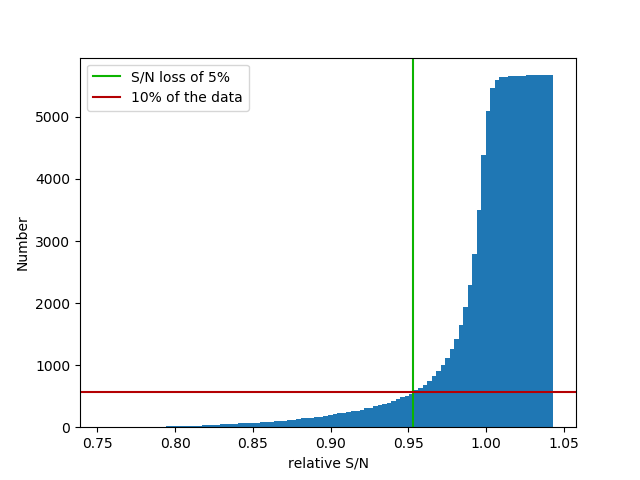
\includegraphics[width=0.75\textwidth]{figures/dist_dash}
\caption{Cumulative distribution of relative S/N. The dash line shows the threshold of 10\% of the whole data set. }\label{his}
\end{figure}

 \paragraph{} To investigate the origin of 10 \% of the synthetic pulsars that have relative S/N less than 95 \%. First, we checked on the relation between period and relative S/N, as shown in Figure \ref{P_twice}. The result shows that the relative S/N is uniformly distributed. Thus, there is no correlation between period and relative S/N.  After that, the relation between relative S/N and acceleration where acceleration is calculated from injected companion mass as shown in Figure \ref{a_twice}. The study shows some correlations between relative S/N and acceleration at some specific accelerations, i.e. 16, 32, and 64 $m/s^2$. We can see that at this acceleration, the algorithm recovers most of the signals. On the other hand, at the accelerations of $\sim$ 14, 25, 50, and 84 $m/s^2$, the relative S/N approaching the local minimum in the plot. Another important parameter that we need to study is the duty cycle $\delta$, as shown in Figure \ref{duty_twice}. The result shows that this error came from a coding mistake that allows the pulse smear to be less than 8 bins instead of 1 bin. The result also shows that most of the low relative S/N detections are originated from pulsars with duty cycle below 6.25 \% or 8 profile bins, which is basically our searching parameter.   
 



 \begin{figure}[h]
\centering
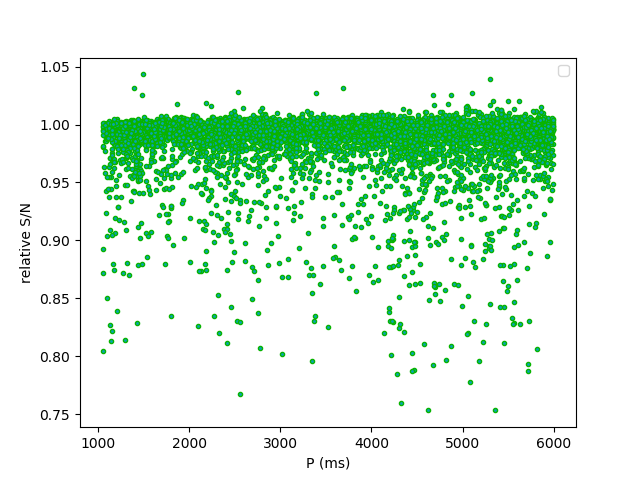
\includegraphics[width=0.80\textwidth]{figures/P_twice}
\caption{Relation between simulated relative S/N and period.  }\label{P_twice}
\end{figure}

\begin{figure}[h!]
\centering
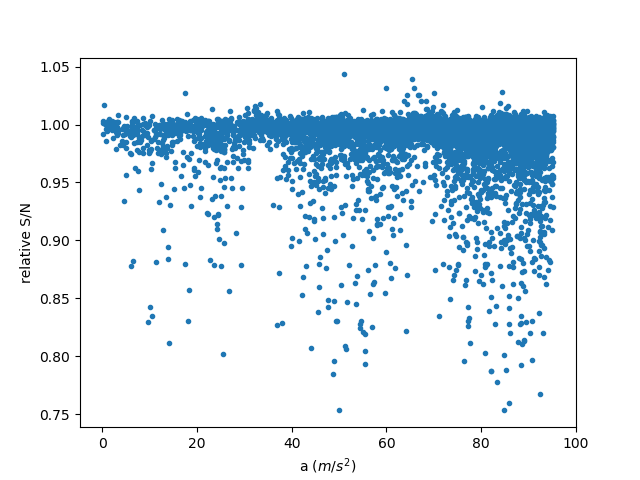
\includegraphics[width=0.80\textwidth]{figures/A}
\caption{Relation between simulated relative S/N and acceleration.  }\label{a_twice}
\end{figure}

\begin{figure}[h!]
\centering
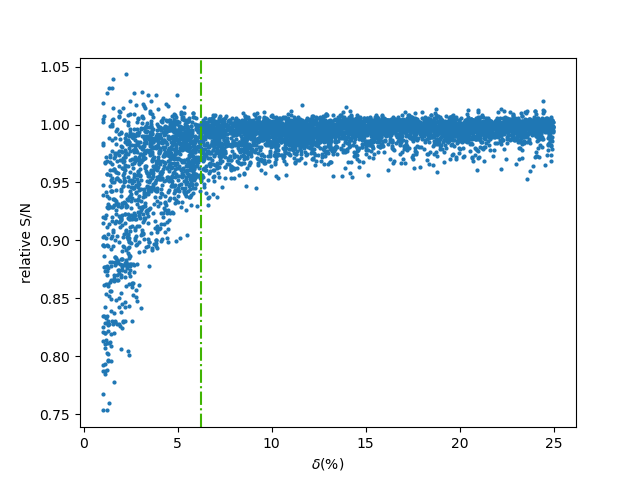
\includegraphics[width=0.80\textwidth]{figures/duty_twice}
\caption{Relation between simulated relative S/N and duty circle $\delta$.}\label{duty_twice}. The green dash-dot line indicate the limit where $\delta \sim 8t_{samp}$.
\end{figure}

\paragraph{} Lastly, as we know that acceleration and duty cycle contribute the detectability of the pipeline, the response pattern between acceleration and duty cycle is investigated, as shown in Figure \ref{a-d}. The result is in line with the previous studies that both of the $\delta$ and acceleration are contributed to the detectability of synthetic pulsars. %However, this implementation is relatively fast and require less number of operation. 
As a conclusion, this method can recover most of the pulsar signals (90 \%) with the S/N loss less than 5\%. This is a mistake that could be corrected in the future. 

\begin{figure}[h!]
\centering
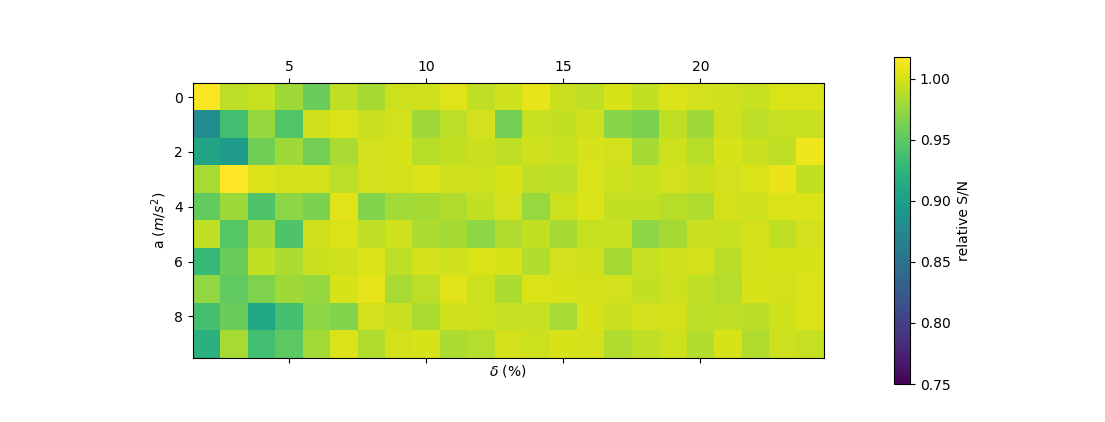
\includegraphics[width=1.0\textwidth]{figures/a-d.png}
\caption{Response patterns of AFFA with duty circle and acceleration .}\label{a-d}
\end{figure}



	\section{New pulsars from AFFA}
  \paragraph{} In this section, I will talk about the preliminary result of applying the AFFA to 122 observations from the HTRU-S low lat data. The full pipeline takes around 12 hours to be complete. Eventhough the pipeline was applied to a small amount of data ($\sim 1 \%$), the pipeline discovered 3 new pulsar candidates. One of them is already confirmed. The follow-ups are re-observed. The pulsar candidates found in the sky were done by observing at the Parkes telescope in the same position in the sky. The follow-ups are essential to confirm that the pulsar candidate is an pulsars-like RFI.  

    \subsection{J1759-1903 missing pulsar from HTRU-S low lat pipeline }
   \paragraph{} As part of the application of \textit{riptide} the FFA search pipeline to the HTRU-S low lat data. This pipeline found a pulsar that was missing from the previous HTRU-S low lat FFT pipeline, reported in \citep{Andrew} and \citep{Ng}. The pulsar was discovered in the HTRU-S Med-lat. The diagnostic plot is shown in Figure \ref{missing}. This pulsar shows the potential of the FFA for discovering missing pulsars from the previous pulsar survey. After the redetection with FFA pipeline, the same pointing is processed with the HTRU-S low lat FFT pipeline. The result from the FFT pipeline shows that this known pulsar is detected in the FFT pipeline but with lower S/N than S/N from the FFA pipeline. Human error might cause this pulsar to be missed.  
       \begin{figure}[h]
\centering
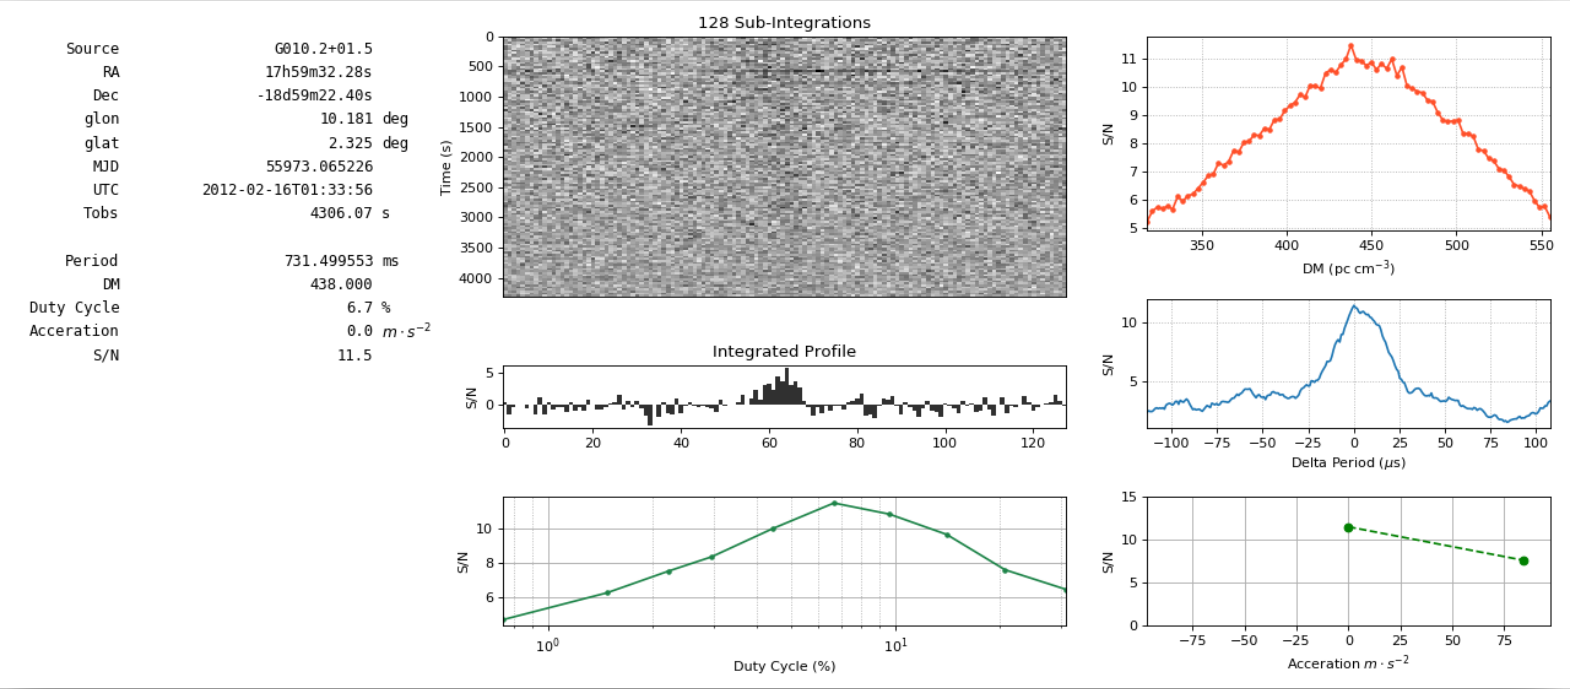
\includegraphics[width=1.0\textwidth]{figures/missing.png}
\caption{Missing pulsar from HTRU-S low lat FFT pipeline}\label{missing}
\end{figure}

    \subsection{J1746-28}
    \paragraph{} The highlight of this thesis is the discovery of J1746-28, the pulsar located at $\sim$ 0.5 degree from the Galactic centre. J1746-28 has a spin period of 1.9 s and a DM of 1290 $pc~cm^{-3}$. The discovered diagnostic plot shown in Figure \ref{J1746}.  Comparing of this pulsar period and DM with all known pulsar in a radius of $1^o$, we found that there is no pulsar in this area which indicates that this pulsar is the newly discovered pulsar. The confirmation of J1746-28 has been done by the Parkes 64m telescope in April 2018 which is approximately seven years from the original detection. The follow up observation using the Parkes telescope shows a detection of the pulsar at the similar period and DM. After that, the observation campaign has begun to observe this pulsar every month for at least 72 minutes to get a better timing solution. Moreover, this pulsar needs a long observation campaign to get timing solution including locating the position of this pulsar in the $P-\dot{P}$ diagram. As mentioned before, location in $P-\dot{P}$ diagram can help us to calculate parameters i.e. $\tau_c$ and $B_{surf}$. 
    \begin{figure}[h]
\centering
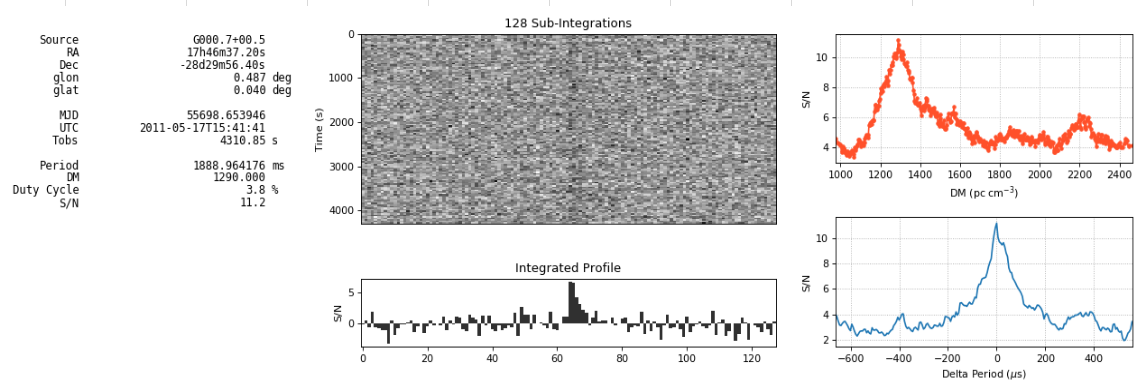
\includegraphics[width=1.0\textwidth]{figures/J1746-28_D.png}
\caption{J1746-28 at discovered pointing plot.}\label{J1746}
\end{figure}
      \subsection{Pulsar candidates}
\paragraph{} Two pulsar candidates are detected in the AFFA pipeline. The first one was found with a period of 523.77s and a DM of 690 $pc~cm^{-3}$. The second pulsar candidate has a period of 1.229s and DM of 222 $pc~cm^{-3}$. Unfortunately, following ups for these pulsars are not successful so far.
%      \paragraph{} Although two pulsar candidates were observed in the same position with the Parkes telescope, but there are no detection on those observations. However, since one of them has known pulsar on the same observation. This known pulsar is detected in original HTRU-S data but not the follow up observation. The non-detection of candidates and a know pulsars  might be originate from an RFI environment on that day that strong enough to change the dynamic range of the observation.
     
\begin{figure}[h]
\centering
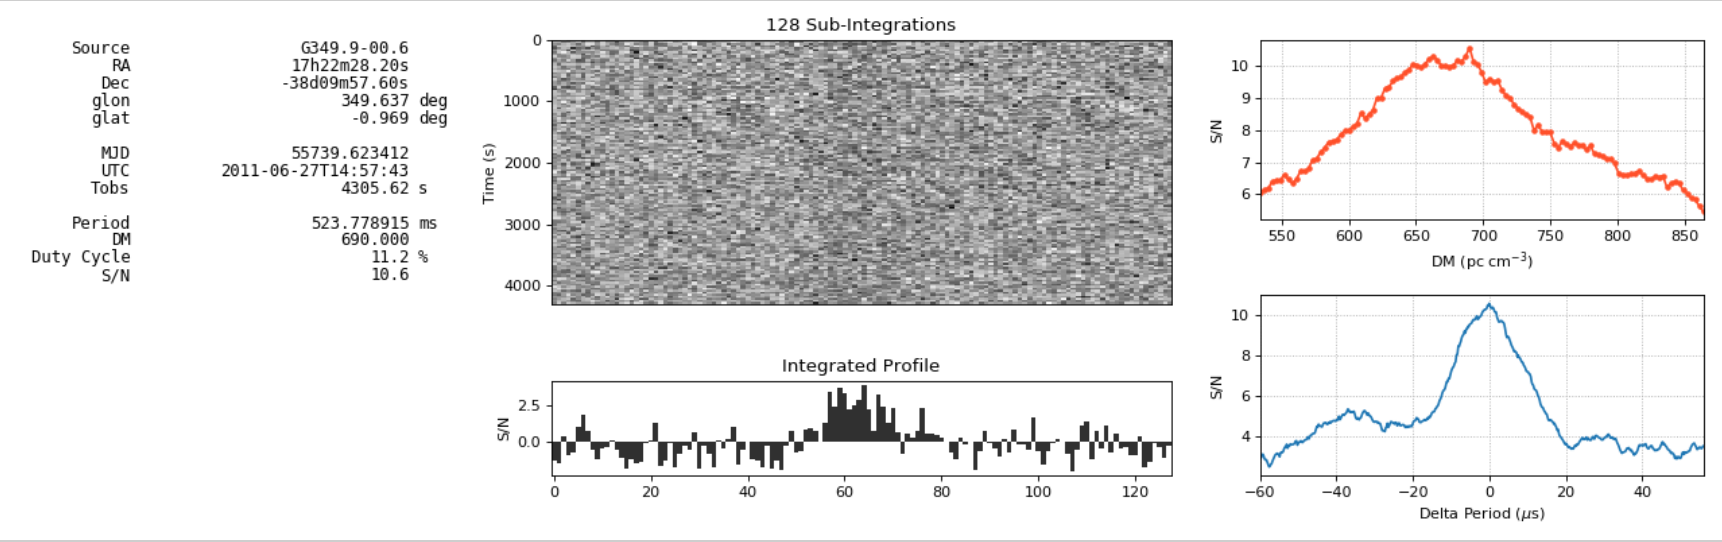
\includegraphics[width=1.0\textwidth]{figures/C1.png}
\caption{Pulsar candidate from from HTRU-S low lat FFT pipeline that has period of 523.77ms }\label{C1}
\end{figure}
 
 \begin{figure}[h]
\centering
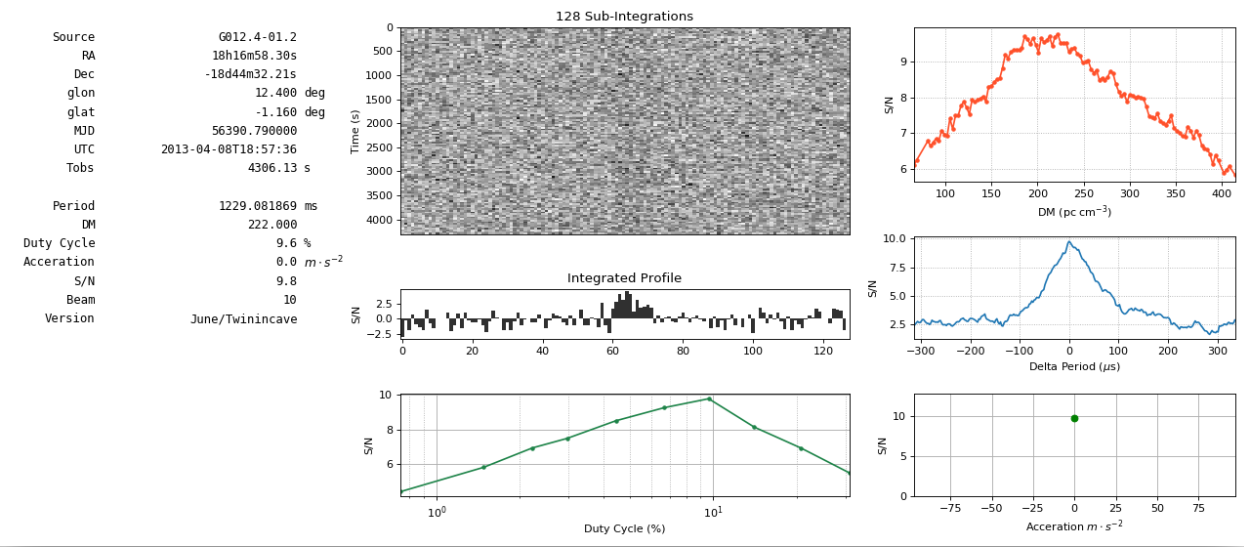
\includegraphics[width=1.0\textwidth]{figures/C2.png}
\caption{Pulsar candidate from from HTRU-S low lat FFT pipeline that has period of 1.22 s with a known pulsar on the same direction.}\label{C2}
\end{figure}
    
\section{Comparison between FFA pipeline and FFT pipeline }
    \paragraph{} To compare the sensitivity between the FFA and the FFT, 122 pointings with known pulsars that were detected in the HTRU-S low lat using the FFT pipeline were applied with the AFFA pipeline. Pointings that were used are combinations of 20 pulsars that were used by \citep{cameron2017investigation} to test the behaviour of the FFA on the real data set and 21 known pulsars selected by the date of observation to avoid selection effect of period S/N and DM. This combination gives test pulsars period well distributed since there are a few known long period pulsars %but also allows us to compare this work to \citep{cameron2017investigation}. 
    The period range of known pulsars is from 190 ms to 6000 ms. The pipeline used the same search parameter as mentioned before. 
    \paragraph{} For the FFT pipeline, the pipeline used \textit{PRESTO} package to mask out the RFI using the package \textit{rfifind} . Then, it de-dispersed using the detected DM, mentioned in \cite{Andrew} and \cite{Ng}. Each time series is resampled with the corresponding acceleration, detected in \cite{Andrew} and \cite{Ng}. After that, each time series is processed through \textit{PRESTO} package \textit{SEEK} and \textit{best} to find the best candidate. The candidate is evaluated by eyes to find the strongest detection with the approximately same period with the period reported in \cite{Andrew} and \cite{Ng}.  The comparison between S/N from the FFA to the FFT is illustrated in Figure \ref{FFA_FFT_real}. The result is in line with the simulation that the FFA is better than the FFT when the period is getting longer.  
    
  \begin{figure}[h!]
\centering
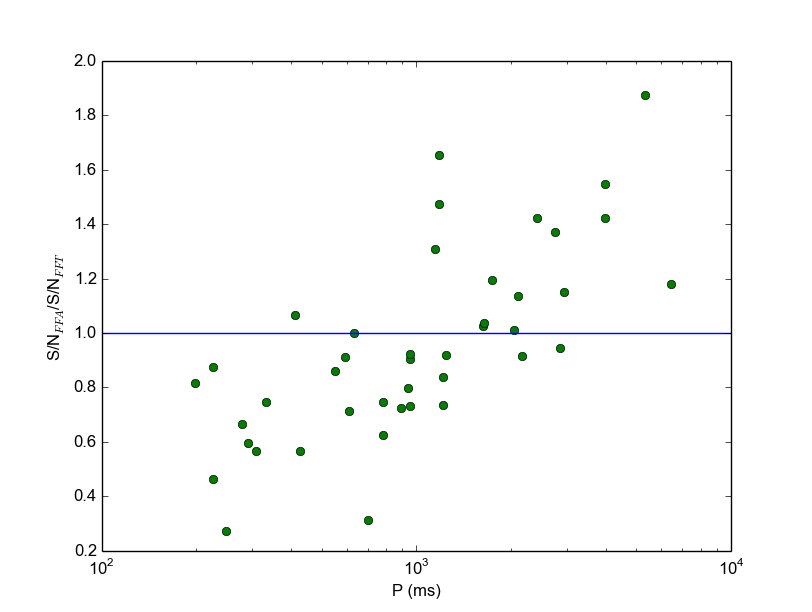
\includegraphics[width=0.85\textwidth]{figures/FFA_FFT_real.png}
\caption{Comparison of the detected S/N using the FFA and the FFT for 41 known pulsars from the HTRU-S low lat survey with spin periods. Periods of pulsars are ranging between 190 ms to 6000 ms. The blue line indicates the limit where S/N$_{FFT}$=S/N$_{FFA}.$}\label{FFA_FFT_real}
\end{figure}

    \section{Confirmation of a pulsar candidates from FAST telescope}
    \paragraph{} As a part of a collaboration between FAST (Five hundred meter Aperture Spherical Telescope) in China for FAST pulsar survey and Effelsberg for the follow up of all of the pulsar candidates. The demonstration of applying the FFA to Effelsberg and the follow-up data off this are shown in Figure \ref{Fast_pulsar}. This pulsar has a period of $\sim$ 5000 ms. The Effelsberg telescope has a strong RFI of $ \sim$ 1000 ms. The $5^{th}$ harmonics of this RFI could effect folded profile of the pulsar. However, the FFA performs matching filter which can separate the pulsar candidate from an RFI, as shown in\ref{fast_rfi}. This shows the potential of the FFA in detecting a weak pulsar that has a spin period near the RFI and also demonstrates the possibility of apply the FFA pipeline to other data sets.     
    
    \begin{figure}[h]
\centering
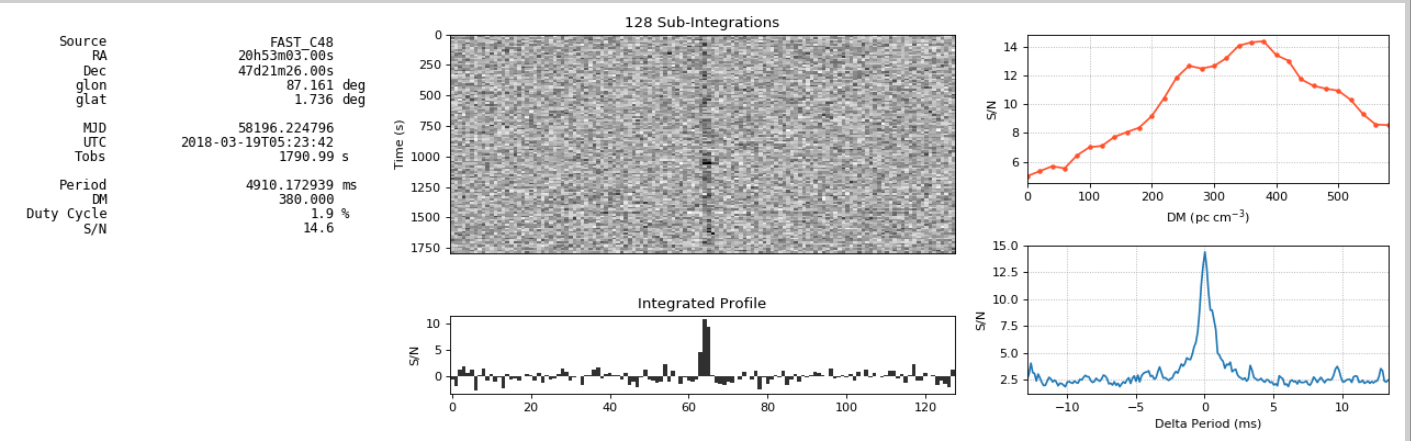
\includegraphics[width=1.0\textwidth]{figures/FAST_pulsar.png}
\caption{Diagnostic plot of newly discovered pulsar}\label{Fast_pulsar}
\end{figure}

    \begin{figure}[h]
\centering
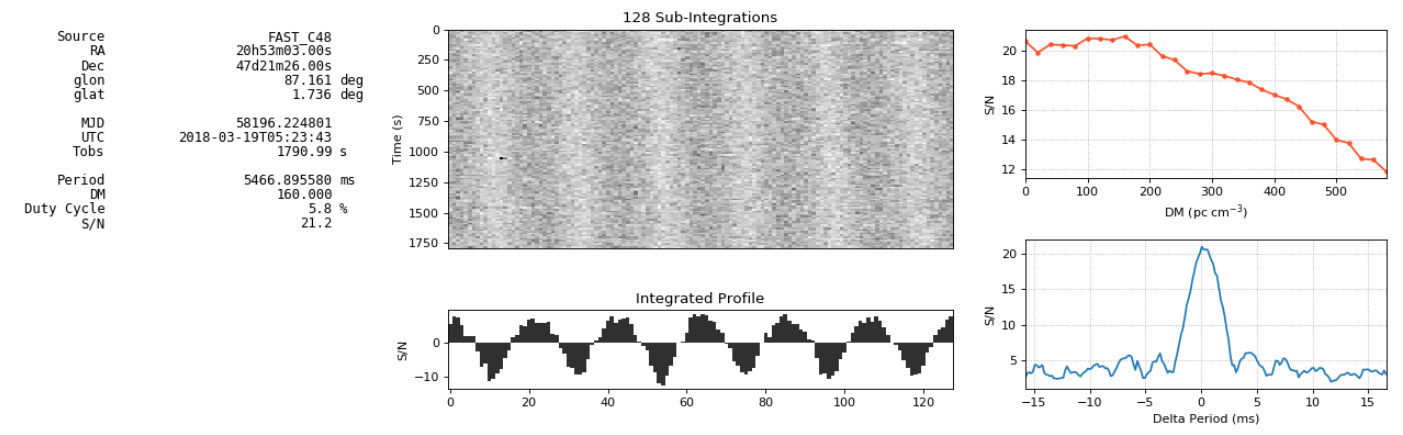
\includegraphics[width=1.0\textwidth]{figures/RFI_fast.png}
\caption{Diagnostic plot of RFI that has a period close to the pulsar.}\label{fast_rfi}
\end{figure}








\iffalse
\section{New RFI mitigation technique} \label{RFI}

     \paragraph{} The list of period bins which is contaminated by RFI will be used as the ``zap table''. The zap table also called as the Birdie list. The zap table is a list of period bins that contaminated with RFI. If the zap table is available before searching, period bins in zap table can be flagged by flagging out corresponding period. The flagging is done by apply the FFT to a time series and then zap out contaminating Fourier bins. Then, the transformed time series is applied by the invest FFT which transformed the Fourier spectrum back to time series. Results from this process are flagged data ready to be used. Moreover, the zap table can also used in the candidate selection by ignore candidates with period bins similar to the RFI. As a result, the zap table need to be available before the searching. %In this chapter, I will present a new method to obtain the zap list before the observation.
     
     \paragraph{} Since RFI creates numerous artificial pulsar candidates, the number distribution of pulsar candidates from each day of observations over the detected periods are studied. The strong periodic RFI will make period bins corresponding to the period of RFI have a large number of candidates. As a result, the periodic RFI is identified by searching for period bins with a high number of candidates. This list of RFI can be used for reprocessing of the data to reduces the number of artificial candidates making fasten the pipeline. Also, the distribution of candidates over long campaigns allows us to study the long time behaviour of RFI. 

     \subsection{RFI mitigation from residual between full data set and mean}
     
    \paragraph{} Over 70 million pulsar candidates which detected in the FFT pipeline that were observed in HTRU-N pulsar survey are used in this work. More detail about the HTRU pulsar survey will be shown in Section \ref{survey}.  This data set contains 193 days of observations ranging from 21$^{st}$ July 2011 to 30$^{th}$ December 2016. The histogram of pulsar candidates distribution over periods for each observation date is made as Figure \ref{RFI_II}. The number distribution of pulsar candidates are normalised by the total number of candidates on the same day to provide the bias from the difference number of the observation in each day.
    \paragraph{} First, the ``RFI profile'' is created by calculating the mean number of candidates in each period bins and subtract that from the full histogram mentioned before as Figure \ref{RFI_profile}. The residual histogram is shown in Figure \ref{RFI_I}. However, this method detects only dynamics RFI because the ``RFI profile'' is already included static RFI. However, this method already shows that the telescope has dynamics RFI. However, since the baseline in the  ``RFI profile'' is not flat especially on short period bins, the short period bins are flagged too much. In this work, I try to flag as less period bin as possible to avoid accidentally flagging real pulsars. 

\begin{figure}[h!] 
\centering
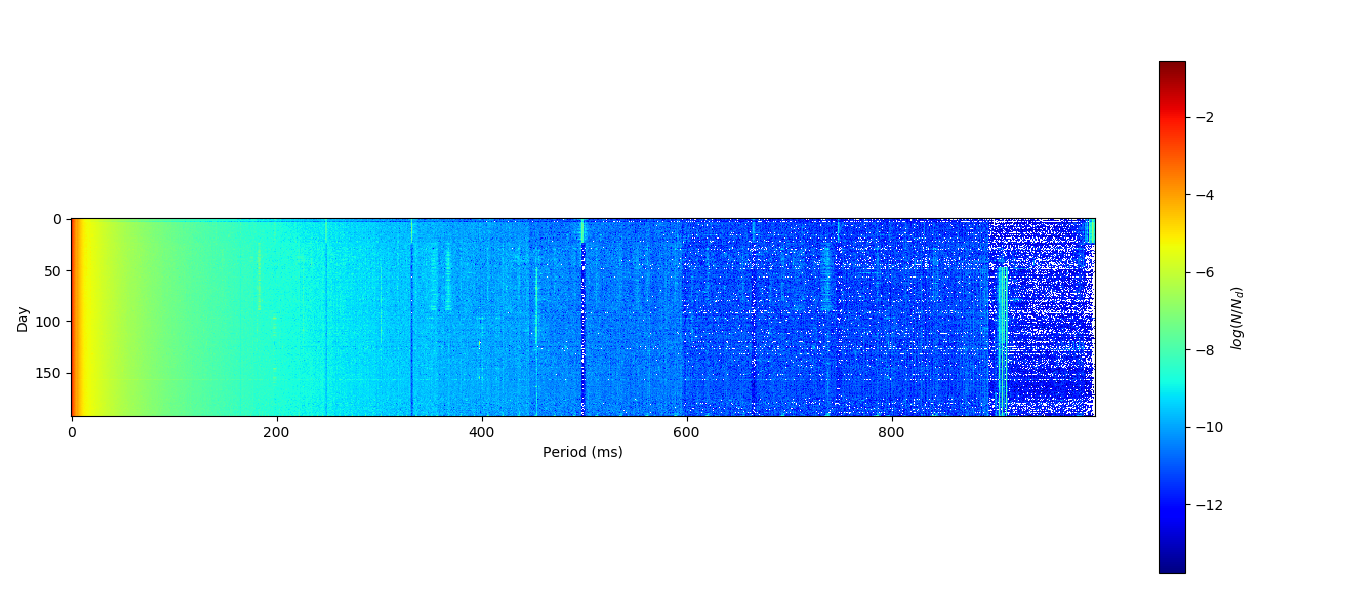
\includegraphics[width=1.0\textwidth]{figures/Full_log.png}
\caption{Distribution of the number of pulsar candidates with the detected period on each observation day. The data is normalised with the total number of candidates on the same day.}
\label{RFI_II}
\end{figure}

\begin{figure}[h!] 
\centering
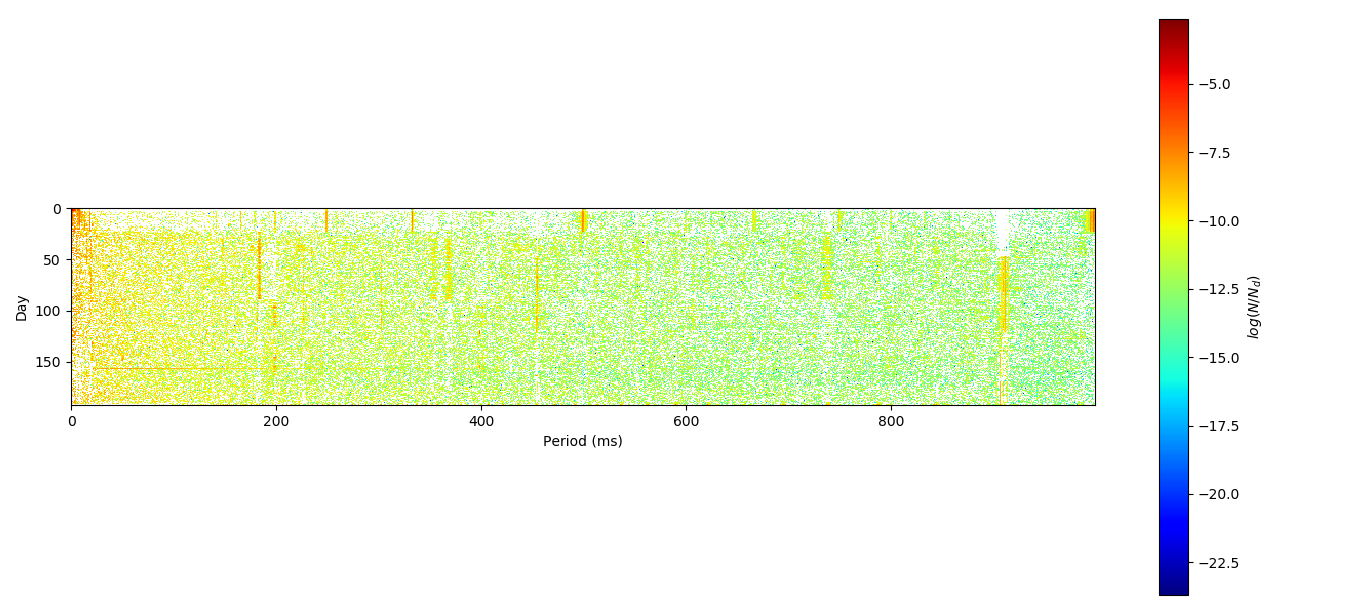
\includegraphics[width=1.0\textwidth]{figures/RFI_mit.png}
\caption{The residual between \ref{RFI_II} and ``RFI profile'' }
\label{RFI_I}
\end{figure}

\begin{figure}[h!] 
\centering
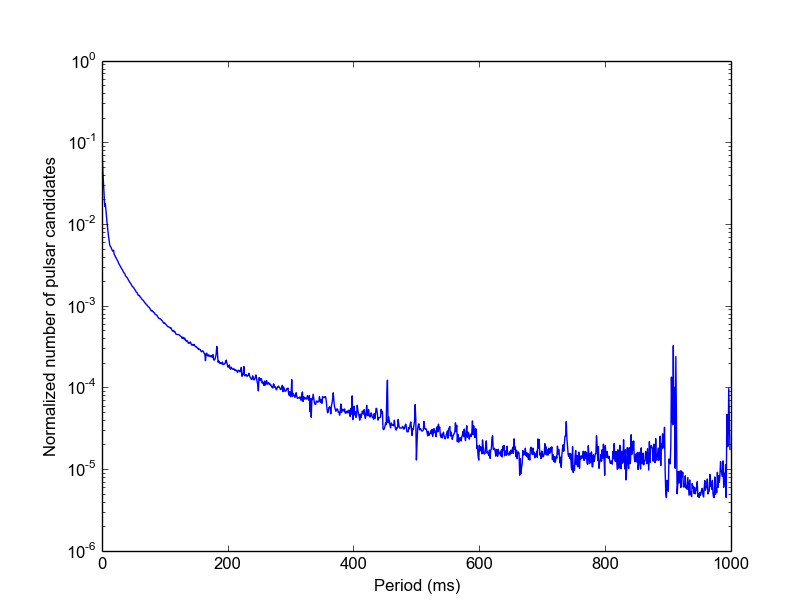
\includegraphics[width=0.7\textwidth]{figures/mean_profile.png}
\caption{The "RFI profile" created from average normalised number of candidates from the whole observation campaign.}
\label{RFI_profile}
\end{figure}

    \subsection{RFI mitigation from statistic distribution of RFI on each day}
    \paragraph{} On the data that has no periodic RFI, the distribution of pulsar candidates are assumed to be the Gaussian distribution. Using the same data set from the previous the section, periodic RFI is identified by detecting and flagging period bins that have the number of candidates bins that not follow the Gaussian distribution. To test how the distribution is similar to the Gaussian distribution, the ``possibility ratio'' is calculated.  The ``possibility ratio'' is a ratio between amplitude at percentile corresponding to $3\sigma$ which is 99.730\%. If the data follows the Gaussian distribution, ratio between each amplitude percentiles and the corresponding standard deviation is unity. This process will be applied repeatedly to the histogram until it follows the Gaussian distribution or different between possibility ratio each iteration step is almost constant.
    \paragraph{} By apply this method to the data on each day. The strong periodic RFI is detected. In this work, the only period range from 200ms - 1000ms is used because the ``RFI profile'' getting flat when the period is more than 200ms. The flat profile is needed to avoid flagging all of the short period candidates. Results agree well with the previous section with only $\sim$ 5 $\%$ of the data flagged. The result of this method is shown at \ref{RFI_III}. RFI lists from this method are generated and will be tested with previous HTRU-N data in the future. 
 
\begin{figure}[h!] 
\centering
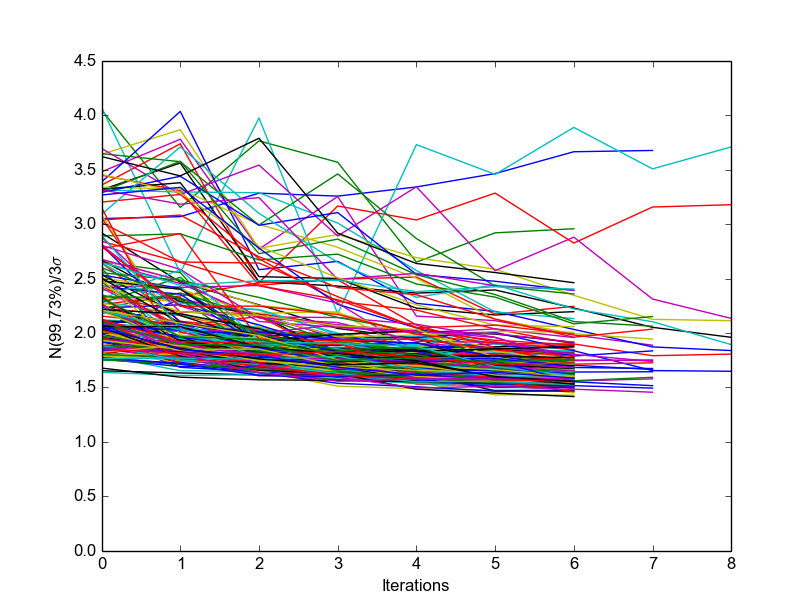
\includegraphics[width=0.7\textwidth]{figures/3sig.png}
\caption{Relation between possibility ratio and iteration for each day. The result shows that most of the data possibility ratio convert to constant number approximately $\sim$ 2. This implies that the pulsar candidates distribution is not perfectly Gaussian distribution. There are a few days that the ratio are not converted which will be studied carefully in the future.}
\label{RFI_3sig}
\end{figure}

\begin{figure}[h!] 
\centering
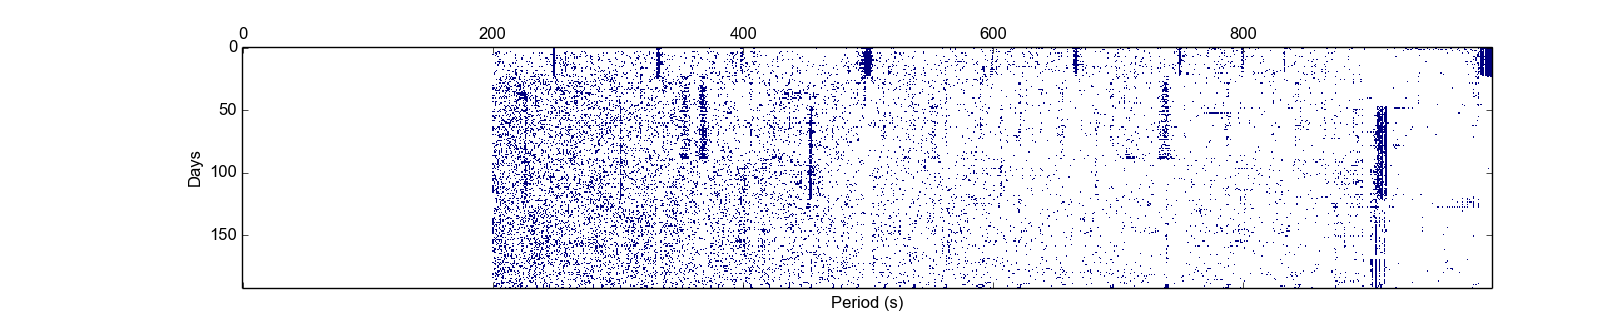
\includegraphics[width=1.0\textwidth]{figures/method2.png}
\caption{Flagged period bins in each day of observation shows the similar result as previous method.}
\label{RFI_III}
\end{figure}
 \newpage
 \subsection{Overview of periodic RFI at Effelsberg telescope }
 \paragraph{} The data shows that the telescope has some RFI in a different epochs. As shown in Figure \ref{RFI_II}, the most prominence RFI has a period of$\sim$ 900ms appeared from day 50 until the end of the observation. Moreover, from day 0-25 which corresponding to 21$^{st}$  July 2011 to 2$^{nd}$  January 2012, there are period bins with have high candidates numbers at $\sim$ 1000, 500, 250 ms and its harmonics. Lastly, period bins around 750 ms and its harmonics appear from days 24 to 89 which corresponding to around 28$^{th}$ February 2012 to 30$^{th}$  December 2016.  
 \fi
\end{document}